\documentclass[border=4pt]{standalone}
\usepackage[T1]{fontenc}
\usepackage{lmodern}
\usepackage{amsmath,amssymb}
\usepackage{tikz}
\usetikzlibrary{positioning,calc}
\usepackage{pgfplots}
\pgfplotsset{compat=1.18}

%% ── Architecture group colours ─────────────────────────────────────────────
\definecolor{myblue}  {RGB}{55, 119, 189}
\definecolor{myred}   {RGB}{210,  70,  70}
\definecolor{mygreen} {RGB}{ 50, 155,  70}
\definecolor{myorange}{RGB}{230, 130,  40}
\definecolor{mygray}  {RGB}{130, 130, 130}

\begin{document}
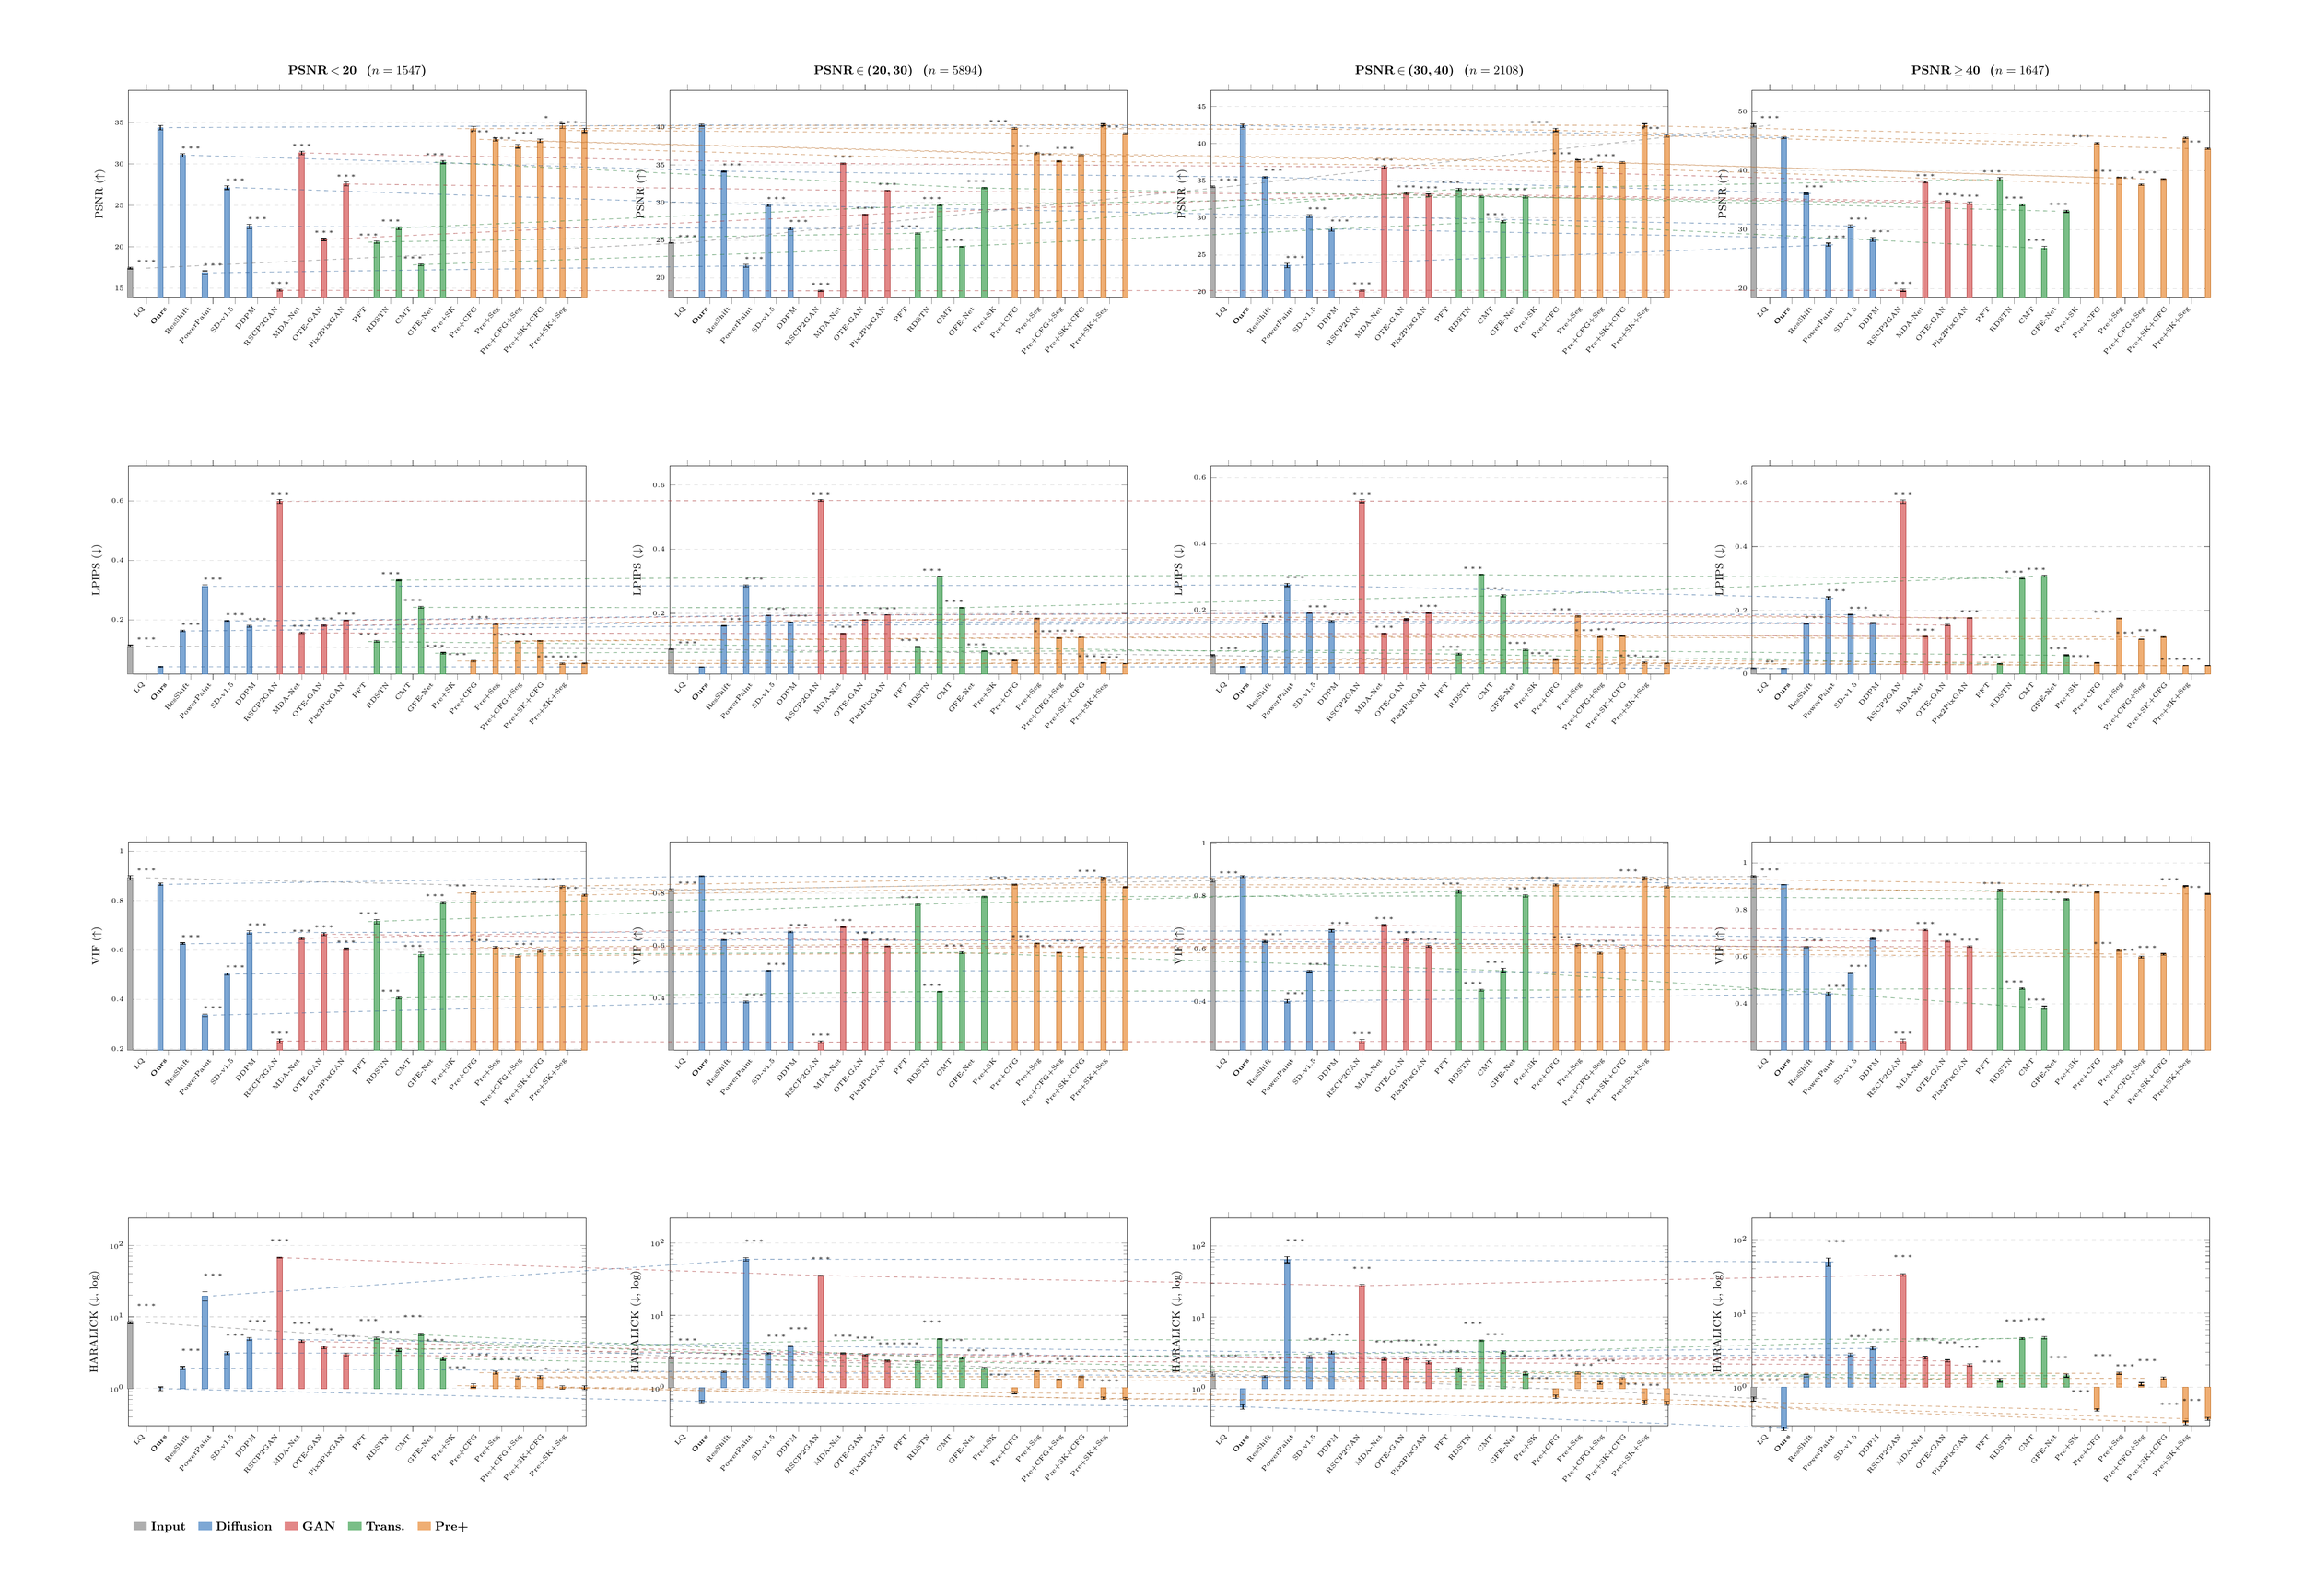
\begin{tikzpicture}[font=\small]
\useasboundingbox (-3.0cm,2.0cm) rectangle (56.3cm,-38.9cm);

% ── PSNR | PSNR<20 ────────────────────────────
\begin{axis}[
  name=ax00,
  at={(0.00cm,0.00cm)},
  anchor=north west,
  width=13.5cm,
  height=7.0cm,
  ybar,
  bar width=4pt,
  xtick={1,...,20},
  xticklabels={{LQ},{\textbf{Ours}},{ResShift},{PowerPaint},{SD-v1.5},{DDPM},{RSCP2GAN},{MDA-Net},{OTE-GAN},{Pix2PixGAN},{PFT},{RDSTN},{CMT},{GFE-Net},{Pre$+$SK},{Pre$+$CFG},{Pre$+$Seg},{Pre$+$CFG$+$Seg},{Pre$+$SK$+$CFG},{Pre$+$SK$+$Seg}},
  xticklabel style={rotate=50, anchor=east, font=\tiny},
  ymin=13.8239,
  ymax=38.9145,
  xmin=0.2,
  xmax=20.8,
  ylabel={PSNR ($\uparrow$)},
  ylabel style={font=\footnotesize},
  ymajorgrids=true,
  grid style={dashed, gray!30},
  tick style={thin},
  every tick label/.style={font=\tiny},
  clip=false,
  scaled y ticks=false,
  y tick label style={font=\tiny, /pgf/number format/fixed,  /pgf/number format/precision=3},
  title={PSNR\,$<$\,20\ \ ($n=1547$)},
  title style={font=\small\bfseries, align=center},
]

\addplot[
  ybar,
  fill=mygray!65, draw=mygray!85!black, line width=0.3pt,
  error bars/.cd, y dir=both, y explicit,
  error bar style={line width=0.6pt, black},
] coordinates {
  (1,17.4350) +- (0.0927,0.0944)
};
\addplot[
  ybar,
  fill=myblue!65, draw=myblue!85!black, line width=0.3pt,
  error bars/.cd, y dir=both, y explicit,
  error bar style={line width=0.6pt, black},
] coordinates {
  (2,34.3978) +- (0.2767,0.2752) (3,31.0604) +- (0.2203,0.2129) (4,16.8826) +- (0.2191,0.2214) (5,27.1577) +- (0.2294,0.2283) (6,22.4661) +- (0.2633,0.2757)
};
\addplot[
  ybar,
  fill=myred!65, draw=myred!85!black, line width=0.3pt,
  error bars/.cd, y dir=both, y explicit,
  error bar style={line width=0.6pt, black},
] coordinates {
  (7,14.7596) +- (0.1263,0.1161) (8,31.3439) +- (0.2117,0.2158) (9,20.9015) +- (0.1489,0.1467) (10,27.5989) +- (0.2285,0.2355)
};
\addplot[
  ybar,
  fill=mygreen!65, draw=mygreen!85!black, line width=0.3pt,
  error bars/.cd, y dir=both, y explicit,
  error bar style={line width=0.6pt, black},
] coordinates {
  (11,20.5757) +- (0.1304,0.1489) (12,22.2468) +- (0.2006,0.1963) (13,17.8322) +- (0.0980,0.1048) (14,30.2316) +- (0.1947,0.1866)
};
\addplot[
  ybar,
  fill=myorange!65, draw=myorange!85!black, line width=0.3pt,
  error bars/.cd, y dir=both, y explicit,
  error bar style={line width=0.6pt, black},
] coordinates {
  (15,34.2753) +- (0.2532,0.2562) (16,32.9795) +- (0.2033,0.1995) (17,32.1345) +- (0.1875,0.2066) (18,32.8004) +- (0.2034,0.1966) (19,34.5833) +- (0.2778,0.2843) (20,34.0578) +- (0.2362,0.2504)
};

\node[above, font=\tiny, inner sep=0pt] at (axis cs:1,18.0312) {$***$};
\coordinate (C0S0M0) at (axis cs:1,17.4350);
\coordinate (C0S0M1) at (axis cs:2,34.3978);
\node[above, font=\tiny, inner sep=0pt] at (axis cs:3,31.7751) {$***$};
\coordinate (C0S0M2) at (axis cs:3,31.0604);
\node[above, font=\tiny, inner sep=0pt] at (axis cs:4,17.6058) {$***$};
\coordinate (C0S0M3) at (axis cs:4,16.8826);
\node[above, font=\tiny, inner sep=0pt] at (axis cs:5,27.8878) {$***$};
\coordinate (C0S0M4) at (axis cs:5,27.1577);
\node[above, font=\tiny, inner sep=0pt] at (axis cs:6,23.2436) {$***$};
\coordinate (C0S0M5) at (axis cs:6,22.4661);
\node[above, font=\tiny, inner sep=0pt] at (axis cs:7,15.3775) {$***$};
\coordinate (C0S0M6) at (axis cs:7,14.7596);
\node[above, font=\tiny, inner sep=0pt] at (axis cs:8,32.0615) {$***$};
\coordinate (C0S0M7) at (axis cs:8,31.3439);
\node[above, font=\tiny, inner sep=0pt] at (axis cs:9,21.5500) {$***$};
\coordinate (C0S0M8) at (axis cs:9,20.9015);
\node[above, font=\tiny, inner sep=0pt] at (axis cs:10,28.3362) {$***$};
\coordinate (C0S0M9) at (axis cs:10,27.5989);
\node[above, font=\tiny, inner sep=0pt] at (axis cs:11,21.2264) {$***$};
\coordinate (C0S0M10) at (axis cs:11,20.5757);
\node[above, font=\tiny, inner sep=0pt] at (axis cs:12,22.9449) {$***$};
\coordinate (C0S0M11) at (axis cs:12,22.2468);
\node[above, font=\tiny, inner sep=0pt] at (axis cs:13,18.4388) {$***$};
\coordinate (C0S0M12) at (axis cs:13,17.8322);
\node[above, font=\tiny, inner sep=0pt] at (axis cs:14,30.9200) {$***$};
\coordinate (C0S0M13) at (axis cs:14,30.2316);
\coordinate (C0S0M14) at (axis cs:15,34.2753);
\node[above, font=\tiny, inner sep=0pt] at (axis cs:16,33.6808) {$***$};
\coordinate (C0S0M15) at (axis cs:16,32.9795);
\node[above, font=\tiny, inner sep=0pt] at (axis cs:17,32.8429) {$***$};
\coordinate (C0S0M16) at (axis cs:17,32.1345);
\node[above, font=\tiny, inner sep=0pt] at (axis cs:18,33.4988) {$***$};
\coordinate (C0S0M17) at (axis cs:18,32.8004);
\node[above, font=\tiny, inner sep=0pt] at (axis cs:19,35.3694) {$*$};
\coordinate (C0S0M18) at (axis cs:19,34.5833);
\node[above, font=\tiny, inner sep=0pt] at (axis cs:20,34.8100) {$***$};
\coordinate (C0S0M19) at (axis cs:20,34.0578);
\end{axis}

% ── PSNR | (20, 30) ────────────────────────────
\begin{axis}[
  name=ax01,
  at={(14.10cm,0.00cm)},
  anchor=north west,
  width=13.5cm,
  height=7.0cm,
  ybar,
  bar width=4pt,
  xtick={1,...,20},
  xticklabels={{LQ},{\textbf{Ours}},{ResShift},{PowerPaint},{SD-v1.5},{DDPM},{RSCP2GAN},{MDA-Net},{OTE-GAN},{Pix2PixGAN},{PFT},{RDSTN},{CMT},{GFE-Net},{Pre$+$SK},{Pre$+$CFG},{Pre$+$Seg},{Pre$+$CFG$+$Seg},{Pre$+$SK$+$CFG},{Pre$+$SK$+$Seg}},
  xticklabel style={rotate=50, anchor=east, font=\tiny},
  ymin=17.3311,
  ymax=44.9200,
  xmin=0.2,
  xmax=20.8,
  ylabel={PSNR ($\uparrow$)},
  ylabel style={font=\footnotesize},
  ymajorgrids=true,
  grid style={dashed, gray!30},
  tick style={thin},
  every tick label/.style={font=\tiny},
  clip=false,
  scaled y ticks=false,
  y tick label style={font=\tiny, /pgf/number format/fixed,  /pgf/number format/precision=3},
  title={PSNR\,$\in$\,(20,\,30)\ \ ($n=5894$)},
  title style={font=\small\bfseries, align=center},
]

\addplot[
  ybar,
  fill=mygray!65, draw=mygray!85!black, line width=0.3pt,
  error bars/.cd, y dir=both, y explicit,
  error bar style={line width=0.6pt, black},
] coordinates {
  (1,24.6726) +- (0.0645,0.0648)
};
\addplot[
  ybar,
  fill=myblue!65, draw=myblue!85!black, line width=0.3pt,
  error bars/.cd, y dir=both, y explicit,
  error bar style={line width=0.6pt, black},
] coordinates {
  (2,40.2814) +- (0.1443,0.1376) (3,34.1509) +- (0.0955,0.0878) (4,21.6230) +- (0.1817,0.1715) (5,29.6414) +- (0.1315,0.1225) (6,26.5674) +- (0.1606,0.1543)
};
\addplot[
  ybar,
  fill=myred!65, draw=myred!85!black, line width=0.3pt,
  error bars/.cd, y dir=both, y explicit,
  error bar style={line width=0.6pt, black},
] coordinates {
  (7,18.2931) +- (0.0720,0.0699) (8,35.1814) +- (0.1001,0.0916) (9,28.4226) +- (0.0839,0.0769) (10,31.5622) +- (0.0988,0.1008)
};
\addplot[
  ybar,
  fill=mygreen!65, draw=mygreen!85!black, line width=0.3pt,
  error bars/.cd, y dir=both, y explicit,
  error bar style={line width=0.6pt, black},
] coordinates {
  (11,25.9174) +- (0.0929,0.0891) (12,29.6493) +- (0.1074,0.1054) (13,24.1557) +- (0.0667,0.0641) (14,31.9448) +- (0.0942,0.0973)
};
\addplot[
  ybar,
  fill=myorange!65, draw=myorange!85!black, line width=0.3pt,
  error bars/.cd, y dir=both, y explicit,
  error bar style={line width=0.6pt, black},
] coordinates {
  (15,39.8539) +- (0.1394,0.1296) (16,36.5726) +- (0.0962,0.0910) (17,35.5114) +- (0.0932,0.0890) (18,36.3194) +- (0.0900,0.0875) (19,40.3402) +- (0.1388,0.1300) (20,39.1515) +- (0.1209,0.1147)
};

\node[above, font=\tiny, inner sep=0pt] at (axis cs:1,25.2892) {$***$};
\coordinate (C0S1M0) at (axis cs:1,24.6726);
\coordinate (C0S1M1) at (axis cs:2,40.2814);
\node[above, font=\tiny, inner sep=0pt] at (axis cs:3,34.7905) {$***$};
\coordinate (C0S1M2) at (axis cs:3,34.1509);
\node[above, font=\tiny, inner sep=0pt] at (axis cs:4,22.3463) {$***$};
\coordinate (C0S1M3) at (axis cs:4,21.6230);
\node[above, font=\tiny, inner sep=0pt] at (axis cs:5,30.3157) {$***$};
\coordinate (C0S1M4) at (axis cs:5,29.6414);
\node[above, font=\tiny, inner sep=0pt] at (axis cs:6,27.2735) {$***$};
\coordinate (C0S1M5) at (axis cs:6,26.5674);
\node[above, font=\tiny, inner sep=0pt] at (axis cs:7,18.9148) {$***$};
\coordinate (C0S1M6) at (axis cs:7,18.2931);
\node[above, font=\tiny, inner sep=0pt] at (axis cs:8,35.8248) {$***$};
\coordinate (C0S1M7) at (axis cs:8,35.1814);
\node[above, font=\tiny, inner sep=0pt] at (axis cs:9,29.0513) {$***$};
\coordinate (C0S1M8) at (axis cs:9,28.4226);
\node[above, font=\tiny, inner sep=0pt] at (axis cs:10,32.2148) {$***$};
\coordinate (C0S1M9) at (axis cs:10,31.5622);
\node[above, font=\tiny, inner sep=0pt] at (axis cs:11,26.5583) {$***$};
\coordinate (C0S1M10) at (axis cs:11,25.9174);
\node[above, font=\tiny, inner sep=0pt] at (axis cs:12,30.3065) {$***$};
\coordinate (C0S1M11) at (axis cs:12,29.6493);
\node[above, font=\tiny, inner sep=0pt] at (axis cs:13,24.7716) {$***$};
\coordinate (C0S1M12) at (axis cs:13,24.1557);
\node[above, font=\tiny, inner sep=0pt] at (axis cs:14,32.5939) {$***$};
\coordinate (C0S1M13) at (axis cs:14,31.9448);
\node[above, font=\tiny, inner sep=0pt] at (axis cs:15,40.5353) {$***$};
\coordinate (C0S1M14) at (axis cs:15,39.8539);
\node[above, font=\tiny, inner sep=0pt] at (axis cs:16,37.2154) {$***$};
\coordinate (C0S1M15) at (axis cs:16,36.5726);
\node[above, font=\tiny, inner sep=0pt] at (axis cs:17,36.1522) {$***$};
\coordinate (C0S1M16) at (axis cs:17,35.5114);
\node[above, font=\tiny, inner sep=0pt] at (axis cs:18,36.9587) {$***$};
\coordinate (C0S1M17) at (axis cs:18,36.3194);
\coordinate (C0S1M18) at (axis cs:19,40.3402);
\node[above, font=\tiny, inner sep=0pt] at (axis cs:20,39.8180) {$***$};
\coordinate (C0S1M19) at (axis cs:20,39.1515);
\end{axis}

% ── PSNR | (30, 40) ────────────────────────────
\begin{axis}[
  name=ax02,
  at={(28.20cm,0.00cm)},
  anchor=north west,
  width=13.5cm,
  height=7.0cm,
  ybar,
  bar width=4pt,
  xtick={1,...,20},
  xticklabels={{LQ},{\textbf{Ours}},{ResShift},{PowerPaint},{SD-v1.5},{DDPM},{RSCP2GAN},{MDA-Net},{OTE-GAN},{Pix2PixGAN},{PFT},{RDSTN},{CMT},{GFE-Net},{Pre$+$SK},{Pre$+$CFG},{Pre$+$Seg},{Pre$+$CFG$+$Seg},{Pre$+$SK$+$CFG},{Pre$+$SK$+$Seg}},
  xticklabel style={rotate=50, anchor=east, font=\tiny},
  ymin=19.1754,
  ymax=47.1984,
  xmin=0.2,
  xmax=20.8,
  ylabel={PSNR ($\uparrow$)},
  ylabel style={font=\footnotesize},
  ymajorgrids=true,
  grid style={dashed, gray!30},
  tick style={thin},
  every tick label/.style={font=\tiny},
  clip=false,
  scaled y ticks=false,
  y tick label style={font=\tiny, /pgf/number format/fixed,  /pgf/number format/precision=3},
  title={PSNR\,$\in$\,(30,\,40)\ \ ($n=2108$)},
  title style={font=\small\bfseries, align=center},
]

\addplot[
  ybar,
  fill=mygray!65, draw=mygray!85!black, line width=0.3pt,
  error bars/.cd, y dir=both, y explicit,
  error bar style={line width=0.6pt, black},
] coordinates {
  (1,34.2027) +- (0.1249,0.1244)
};
\addplot[
  ybar,
  fill=myblue!65, draw=myblue!85!black, line width=0.3pt,
  error bars/.cd, y dir=both, y explicit,
  error bar style={line width=0.6pt, black},
] coordinates {
  (2,42.4223) +- (0.2220,0.2194) (3,35.4577) +- (0.1141,0.1195) (4,23.5773) +- (0.3124,0.3033) (5,30.2391) +- (0.2033,0.2074) (6,28.4687) +- (0.2767,0.2816)
};
\addplot[
  ybar,
  fill=myred!65, draw=myred!85!black, line width=0.3pt,
  error bars/.cd, y dir=both, y explicit,
  error bar style={line width=0.6pt, black},
] coordinates {
  (7,20.2100) +- (0.1306,0.1216) (8,36.8301) +- (0.1352,0.1363) (9,33.2829) +- (0.1138,0.1049) (10,33.0513) +- (0.1699,0.1674)
};
\addplot[
  ybar,
  fill=mygreen!65, draw=mygreen!85!black, line width=0.3pt,
  error bars/.cd, y dir=both, y explicit,
  error bar style={line width=0.6pt, black},
] coordinates {
  (11,33.8006) +- (0.1553,0.1568) (12,32.8481) +- (0.1302,0.1331) (13,29.4704) +- (0.2043,0.1832) (14,32.8405) +- (0.1662,0.1622)
};
\addplot[
  ybar,
  fill=myorange!65, draw=myorange!85!black, line width=0.3pt,
  error bars/.cd, y dir=both, y explicit,
  error bar style={line width=0.6pt, black},
] coordinates {
  (15,41.8335) +- (0.2077,0.2099) (16,37.6688) +- (0.1469,0.1477) (17,36.8208) +- (0.1358,0.1427) (18,37.4468) +- (0.1340,0.1415) (19,42.4587) +- (0.2264,0.2199) (20,41.0558) +- (0.1929,0.1869)
};

\node[above, font=\tiny, inner sep=0pt] at (axis cs:1,34.8876) {$***$};
\coordinate (C0S2M0) at (axis cs:1,34.2027);
\coordinate (C0S2M1) at (axis cs:2,42.4223);
\node[above, font=\tiny, inner sep=0pt] at (axis cs:3,36.1377) {$***$};
\coordinate (C0S2M2) at (axis cs:3,35.4577);
\node[above, font=\tiny, inner sep=0pt] at (axis cs:4,24.4411) {$***$};
\coordinate (C0S2M3) at (axis cs:4,23.5773);
\node[above, font=\tiny, inner sep=0pt] at (axis cs:5,31.0070) {$***$};
\coordinate (C0S2M4) at (axis cs:5,30.2391);
\node[above, font=\tiny, inner sep=0pt] at (axis cs:6,29.3108) {$***$};
\coordinate (C0S2M5) at (axis cs:6,28.4687);
\node[above, font=\tiny, inner sep=0pt] at (axis cs:7,20.8921) {$***$};
\coordinate (C0S2M6) at (axis cs:7,20.2100);
\node[above, font=\tiny, inner sep=0pt] at (axis cs:8,37.5269) {$***$};
\coordinate (C0S2M7) at (axis cs:8,36.8301);
\node[above, font=\tiny, inner sep=0pt] at (axis cs:9,33.9483) {$***$};
\coordinate (C0S2M8) at (axis cs:9,33.2829);
\node[above, font=\tiny, inner sep=0pt] at (axis cs:10,33.7792) {$***$};
\coordinate (C0S2M9) at (axis cs:10,33.0513);
\node[above, font=\tiny, inner sep=0pt] at (axis cs:11,34.5179) {$***$};
\coordinate (C0S2M10) at (axis cs:11,33.8006);
\node[above, font=\tiny, inner sep=0pt] at (axis cs:12,33.5417) {$***$};
\coordinate (C0S2M11) at (axis cs:12,32.8481);
\node[above, font=\tiny, inner sep=0pt] at (axis cs:13,30.2141) {$***$};
\coordinate (C0S2M12) at (axis cs:13,29.4704);
\node[above, font=\tiny, inner sep=0pt] at (axis cs:14,33.5632) {$***$};
\coordinate (C0S2M13) at (axis cs:14,32.8405);
\node[above, font=\tiny, inner sep=0pt] at (axis cs:15,42.6039) {$***$};
\coordinate (C0S2M14) at (axis cs:15,41.8335);
\node[above, font=\tiny, inner sep=0pt] at (axis cs:16,38.3770) {$***$};
\coordinate (C0S2M15) at (axis cs:16,37.6688);
\node[above, font=\tiny, inner sep=0pt] at (axis cs:17,37.5240) {$***$};
\coordinate (C0S2M16) at (axis cs:17,36.8208);
\node[above, font=\tiny, inner sep=0pt] at (axis cs:18,38.1488) {$***$};
\coordinate (C0S2M17) at (axis cs:18,37.4468);
\coordinate (C0S2M18) at (axis cs:19,42.4587);
\node[above, font=\tiny, inner sep=0pt] at (axis cs:20,41.8032) {$***$};
\coordinate (C0S2M19) at (axis cs:20,41.0558);
\end{axis}

% ── PSNR | (40, 40+) ────────────────────────────
\begin{axis}[
  name=ax03,
  at={(42.30cm,0.00cm)},
  anchor=north west,
  width=13.5cm,
  height=7.0cm,
  ybar,
  bar width=4pt,
  xtick={1,...,20},
  xticklabels={{LQ},{\textbf{Ours}},{ResShift},{PowerPaint},{SD-v1.5},{DDPM},{RSCP2GAN},{MDA-Net},{OTE-GAN},{Pix2PixGAN},{PFT},{RDSTN},{CMT},{GFE-Net},{Pre$+$SK},{Pre$+$CFG},{Pre$+$Seg},{Pre$+$CFG$+$Seg},{Pre$+$SK$+$CFG},{Pre$+$SK$+$Seg}},
  xticklabel style={rotate=50, anchor=east, font=\tiny},
  ymin=18.3916,
  ymax=53.6419,
  xmin=0.2,
  xmax=20.8,
  ylabel={PSNR ($\uparrow$)},
  ylabel style={font=\footnotesize},
  ymajorgrids=true,
  grid style={dashed, gray!30},
  tick style={thin},
  every tick label/.style={font=\tiny},
  clip=false,
  scaled y ticks=false,
  y tick label style={font=\tiny, /pgf/number format/fixed,  /pgf/number format/precision=3},
  title={PSNR\,$\geq$\,40\ \ ($n=1647$)},
  title style={font=\small\bfseries, align=center},
]

\addplot[
  ybar,
  fill=mygray!65, draw=mygray!85!black, line width=0.3pt,
  error bars/.cd, y dir=both, y explicit,
  error bar style={line width=0.6pt, black},
] coordinates {
  (1,47.6937) +- (0.2652,0.2627)
};
\addplot[
  ybar,
  fill=myblue!65, draw=myblue!85!black, line width=0.3pt,
  error bars/.cd, y dir=both, y explicit,
  error bar style={line width=0.6pt, black},
] coordinates {
  (2,45.5607) +- (0.1439,0.1174) (3,36.0989) +- (0.1266,0.1254) (4,27.4519) +- (0.2896,0.2560) (5,30.5805) +- (0.2890,0.2224) (6,28.3515) +- (0.3800,0.3383)
};
\addplot[
  ybar,
  fill=myred!65, draw=myred!85!black, line width=0.3pt,
  error bars/.cd, y dir=both, y explicit,
  error bar style={line width=0.6pt, black},
] coordinates {
  (7,19.7038) +- (0.1751,0.1753) (8,38.0191) +- (0.1364,0.1264) (9,34.7999) +- (0.1375,0.1239) (10,34.4924) +- (0.2202,0.1957)
};
\addplot[
  ybar,
  fill=mygreen!65, draw=mygreen!85!black, line width=0.3pt,
  error bars/.cd, y dir=both, y explicit,
  error bar style={line width=0.6pt, black},
] coordinates {
  (11,38.5156) +- (0.3115,0.2984) (12,34.2079) +- (0.1745,0.1486) (13,26.8892) +- (0.2653,0.2601) (14,33.1113) +- (0.1967,0.1906)
};
\addplot[
  ybar,
  fill=myorange!65, draw=myorange!85!black, line width=0.3pt,
  error bars/.cd, y dir=both, y explicit,
  error bar style={line width=0.6pt, black},
] coordinates {
  (15,44.6238) +- (0.1240,0.1156) (16,38.8312) +- (0.1105,0.1071) (17,37.6256) +- (0.1461,0.1309) (18,38.5721) +- (0.1028,0.1054) (19,45.5472) +- (0.1371,0.1236) (20,43.7301) +- (0.1155,0.1118)
};

\node[above, font=\tiny, inner sep=0pt] at (axis cs:1,48.6614) {$***$};
\coordinate (C0S3M0) at (axis cs:1,47.6937);
\coordinate (C0S3M1) at (axis cs:2,45.5607);
\node[above, font=\tiny, inner sep=0pt] at (axis cs:3,36.9293) {$***$};
\coordinate (C0S3M2) at (axis cs:3,36.0989);
\node[above, font=\tiny, inner sep=0pt] at (axis cs:4,28.4129) {$***$};
\coordinate (C0S3M3) at (axis cs:4,27.4519);
\node[above, font=\tiny, inner sep=0pt] at (axis cs:5,31.5079) {$***$};
\coordinate (C0S3M4) at (axis cs:5,30.5805);
\node[above, font=\tiny, inner sep=0pt] at (axis cs:6,29.3948) {$***$};
\coordinate (C0S3M5) at (axis cs:6,28.3515);
\node[above, font=\tiny, inner sep=0pt] at (axis cs:7,20.5841) {$***$};
\coordinate (C0S3M6) at (axis cs:7,19.7038);
\node[above, font=\tiny, inner sep=0pt] at (axis cs:8,38.8505) {$***$};
\coordinate (C0S3M7) at (axis cs:8,38.0191);
\node[above, font=\tiny, inner sep=0pt] at (axis cs:9,35.6288) {$***$};
\coordinate (C0S3M8) at (axis cs:9,34.7999);
\node[above, font=\tiny, inner sep=0pt] at (axis cs:10,35.3931) {$***$};
\coordinate (C0S3M9) at (axis cs:10,34.4924);
\node[above, font=\tiny, inner sep=0pt] at (axis cs:11,39.5190) {$***$};
\coordinate (C0S3M10) at (axis cs:11,38.5156);
\node[above, font=\tiny, inner sep=0pt] at (axis cs:12,35.0615) {$***$};
\coordinate (C0S3M11) at (axis cs:12,34.2079);
\node[above, font=\tiny, inner sep=0pt] at (axis cs:13,27.8543) {$***$};
\coordinate (C0S3M12) at (axis cs:13,26.8892);
\node[above, font=\tiny, inner sep=0pt] at (axis cs:14,34.0069) {$***$};
\coordinate (C0S3M13) at (axis cs:14,33.1113);
\node[above, font=\tiny, inner sep=0pt] at (axis cs:15,45.4444) {$***$};
\coordinate (C0S3M14) at (axis cs:15,44.6238);
\node[above, font=\tiny, inner sep=0pt] at (axis cs:16,39.6433) {$***$};
\coordinate (C0S3M15) at (axis cs:16,38.8312);
\node[above, font=\tiny, inner sep=0pt] at (axis cs:17,38.4615) {$***$};
\coordinate (C0S3M16) at (axis cs:17,37.6256);
\node[above, font=\tiny, inner sep=0pt] at (axis cs:18,39.3825) {$***$};
\coordinate (C0S3M17) at (axis cs:18,38.5721);
\coordinate (C0S3M18) at (axis cs:19,45.5472);
\node[above, font=\tiny, inner sep=0pt] at (axis cs:20,44.5469) {$***$};
\coordinate (C0S3M19) at (axis cs:20,43.7301);
\end{axis}

% ── LPIPS | PSNR<20 ────────────────────────────
\begin{axis}[
  name=ax10,
  at={(0.00cm,-9.80cm)},
  anchor=north west,
  width=13.5cm,
  height=7.0cm,
  ybar,
  bar width=4pt,
  xtick={1,...,20},
  xticklabels={{LQ},{\textbf{Ours}},{ResShift},{PowerPaint},{SD-v1.5},{DDPM},{RSCP2GAN},{MDA-Net},{OTE-GAN},{Pix2PixGAN},{PFT},{RDSTN},{CMT},{GFE-Net},{Pre$+$SK},{Pre$+$CFG},{Pre$+$Seg},{Pre$+$CFG$+$Seg},{Pre$+$SK$+$CFG},{Pre$+$SK$+$Seg}},
  xticklabel style={rotate=50, anchor=east, font=\tiny},
  ymin=0.0182,
  ymax=0.7174,
  xmin=0.2,
  xmax=20.8,
  ylabel={LPIPS ($\downarrow$)},
  ylabel style={font=\footnotesize},
  ymajorgrids=true,
  grid style={dashed, gray!30},
  tick style={thin},
  every tick label/.style={font=\tiny},
  clip=false,
  scaled y ticks=false,
  y tick label style={font=\tiny, /pgf/number format/fixed,  /pgf/number format/precision=3},
]

\addplot[
  ybar,
  fill=mygray!65, draw=mygray!85!black, line width=0.3pt,
  error bars/.cd, y dir=both, y explicit,
  error bar style={line width=0.6pt, black},
] coordinates {
  (1,0.1121) +- (0.0033,0.0035)
};
\addplot[
  ybar,
  fill=myblue!65, draw=myblue!85!black, line width=0.3pt,
  error bars/.cd, y dir=both, y explicit,
  error bar style={line width=0.6pt, black},
] coordinates {
  (2,0.0427) +- (0.0019,0.0021) (3,0.1631) +- (0.0018,0.0018) (4,0.3131) +- (0.0049,0.0045) (5,0.1964) +- (0.0017,0.0017) (6,0.1788) +- (0.0027,0.0028)
};
\addplot[
  ybar,
  fill=myred!65, draw=myred!85!black, line width=0.3pt,
  error bars/.cd, y dir=both, y explicit,
  error bar style={line width=0.6pt, black},
] coordinates {
  (7,0.5982) +- (0.0066,0.0064) (8,0.1562) +- (0.0024,0.0022) (9,0.1816) +- (0.0026,0.0027) (10,0.1983) +- (0.0022,0.0022)
};
\addplot[
  ybar,
  fill=mygreen!65, draw=mygreen!85!black, line width=0.3pt,
  error bars/.cd, y dir=both, y explicit,
  error bar style={line width=0.6pt, black},
] coordinates {
  (11,0.1273) +- (0.0032,0.0032) (12,0.3338) +- (0.0020,0.0019) (13,0.2425) +- (0.0040,0.0038) (14,0.0882) +- (0.0026,0.0028)
};
\addplot[
  ybar,
  fill=myorange!65, draw=myorange!85!black, line width=0.3pt,
  error bars/.cd, y dir=both, y explicit,
  error bar style={line width=0.6pt, black},
] coordinates {
  (15,0.0620) +- (0.0022,0.0023) (16,0.1859) +- (0.0023,0.0021) (17,0.1278) +- (0.0018,0.0018) (18,0.1299) +- (0.0019,0.0017) (19,0.0533) +- (0.0022,0.0023) (20,0.0542) +- (0.0020,0.0021)
};

\node[above, font=\tiny, inner sep=0pt] at (axis cs:1,0.1296) {$***$};
\coordinate (C1S0M0) at (axis cs:1,0.1121);
\coordinate (C1S0M1) at (axis cs:2,0.0427);
\node[above, font=\tiny, inner sep=0pt] at (axis cs:3,0.1789) {$***$};
\coordinate (C1S0M2) at (axis cs:3,0.1631);
\node[above, font=\tiny, inner sep=0pt] at (axis cs:4,0.3316) {$***$};
\coordinate (C1S0M3) at (axis cs:4,0.3131);
\node[above, font=\tiny, inner sep=0pt] at (axis cs:5,0.2121) {$***$};
\coordinate (C1S0M4) at (axis cs:5,0.1964);
\node[above, font=\tiny, inner sep=0pt] at (axis cs:6,0.1956) {$***$};
\coordinate (C1S0M5) at (axis cs:6,0.1788);
\node[above, font=\tiny, inner sep=0pt] at (axis cs:7,0.6186) {$***$};
\coordinate (C1S0M6) at (axis cs:7,0.5982);
\node[above, font=\tiny, inner sep=0pt] at (axis cs:8,0.1724) {$***$};
\coordinate (C1S0M7) at (axis cs:8,0.1562);
\node[above, font=\tiny, inner sep=0pt] at (axis cs:9,0.1983) {$***$};
\coordinate (C1S0M8) at (axis cs:9,0.1816);
\node[above, font=\tiny, inner sep=0pt] at (axis cs:10,0.2145) {$***$};
\coordinate (C1S0M9) at (axis cs:10,0.1983);
\node[above, font=\tiny, inner sep=0pt] at (axis cs:11,0.1445) {$***$};
\coordinate (C1S0M10) at (axis cs:11,0.1273);
\node[above, font=\tiny, inner sep=0pt] at (axis cs:12,0.3497) {$***$};
\coordinate (C1S0M11) at (axis cs:12,0.3338);
\node[above, font=\tiny, inner sep=0pt] at (axis cs:13,0.2603) {$***$};
\coordinate (C1S0M12) at (axis cs:13,0.2425);
\node[above, font=\tiny, inner sep=0pt] at (axis cs:14,0.1050) {$***$};
\coordinate (C1S0M13) at (axis cs:14,0.0882);
\node[above, font=\tiny, inner sep=0pt] at (axis cs:15,0.0783) {$***$};
\coordinate (C1S0M14) at (axis cs:15,0.0620);
\node[above, font=\tiny, inner sep=0pt] at (axis cs:16,0.2020) {$***$};
\coordinate (C1S0M15) at (axis cs:16,0.1859);
\node[above, font=\tiny, inner sep=0pt] at (axis cs:17,0.1436) {$***$};
\coordinate (C1S0M16) at (axis cs:17,0.1278);
\node[above, font=\tiny, inner sep=0pt] at (axis cs:18,0.1456) {$***$};
\coordinate (C1S0M17) at (axis cs:18,0.1299);
\node[above, font=\tiny, inner sep=0pt] at (axis cs:19,0.0696) {$***$};
\coordinate (C1S0M18) at (axis cs:19,0.0533);
\node[above, font=\tiny, inner sep=0pt] at (axis cs:20,0.0703) {$***$};
\coordinate (C1S0M19) at (axis cs:20,0.0542);
\end{axis}

% ── LPIPS | (20, 30) ────────────────────────────
\begin{axis}[
  name=ax11,
  at={(14.10cm,-9.80cm)},
  anchor=north west,
  width=13.5cm,
  height=7.0cm,
  ybar,
  bar width=4pt,
  xtick={1,...,20},
  xticklabels={{LQ},{\textbf{Ours}},{ResShift},{PowerPaint},{SD-v1.5},{DDPM},{RSCP2GAN},{MDA-Net},{OTE-GAN},{Pix2PixGAN},{PFT},{RDSTN},{CMT},{GFE-Net},{Pre$+$SK},{Pre$+$CFG},{Pre$+$Seg},{Pre$+$CFG$+$Seg},{Pre$+$SK$+$CFG},{Pre$+$SK$+$Seg}},
  xticklabel style={rotate=50, anchor=east, font=\tiny},
  ymin=0.0108,
  ymax=0.6592,
  xmin=0.2,
  xmax=20.8,
  ylabel={LPIPS ($\downarrow$)},
  ylabel style={font=\footnotesize},
  ymajorgrids=true,
  grid style={dashed, gray!30},
  tick style={thin},
  every tick label/.style={font=\tiny},
  clip=false,
  scaled y ticks=false,
  y tick label style={font=\tiny, /pgf/number format/fixed,  /pgf/number format/precision=3},
]

\addplot[
  ybar,
  fill=mygray!65, draw=mygray!85!black, line width=0.3pt,
  error bars/.cd, y dir=both, y explicit,
  error bar style={line width=0.6pt, black},
] coordinates {
  (1,0.0885) +- (0.0018,0.0018)
};
\addplot[
  ybar,
  fill=myblue!65, draw=myblue!85!black, line width=0.3pt,
  error bars/.cd, y dir=both, y explicit,
  error bar style={line width=0.6pt, black},
] coordinates {
  (2,0.0328) +- (0.0011,0.0011) (3,0.1614) +- (0.0009,0.0010) (4,0.2860) +- (0.0030,0.0028) (5,0.1935) +- (0.0008,0.0008) (6,0.1720) +- (0.0014,0.0014)
};
\addplot[
  ybar,
  fill=myred!65, draw=myred!85!black, line width=0.3pt,
  error bars/.cd, y dir=both, y explicit,
  error bar style={line width=0.6pt, black},
] coordinates {
  (7,0.5516) +- (0.0030,0.0030) (8,0.1370) +- (0.0013,0.0013) (9,0.1789) +- (0.0014,0.0014) (10,0.1955) +- (0.0012,0.0012)
};
\addplot[
  ybar,
  fill=mygreen!65, draw=mygreen!85!black, line width=0.3pt,
  error bars/.cd, y dir=both, y explicit,
  error bar style={line width=0.6pt, black},
] coordinates {
  (11,0.0952) +- (0.0018,0.0019) (12,0.3152) +- (0.0009,0.0009) (13,0.2174) +- (0.0018,0.0017) (14,0.0817) +- (0.0016,0.0017)
};
\addplot[
  ybar,
  fill=myorange!65, draw=myorange!85!black, line width=0.3pt,
  error bars/.cd, y dir=both, y explicit,
  error bar style={line width=0.6pt, black},
] coordinates {
  (15,0.0538) +- (0.0013,0.0013) (16,0.1841) +- (0.0012,0.0012) (17,0.1232) +- (0.0009,0.0010) (18,0.1251) +- (0.0009,0.0009) (19,0.0450) +- (0.0013,0.0014) (20,0.0435) +- (0.0011,0.0011)
};

\node[above, font=\tiny, inner sep=0pt] at (axis cs:1,0.1033) {$***$};
\coordinate (C1S1M0) at (axis cs:1,0.0885);
\coordinate (C1S1M1) at (axis cs:2,0.0328);
\node[above, font=\tiny, inner sep=0pt] at (axis cs:3,0.1754) {$***$};
\coordinate (C1S1M2) at (axis cs:3,0.1614);
\node[above, font=\tiny, inner sep=0pt] at (axis cs:4,0.3018) {$***$};
\coordinate (C1S1M3) at (axis cs:4,0.2860);
\node[above, font=\tiny, inner sep=0pt] at (axis cs:5,0.2073) {$***$};
\coordinate (C1S1M4) at (axis cs:5,0.1935);
\node[above, font=\tiny, inner sep=0pt] at (axis cs:6,0.1864) {$***$};
\coordinate (C1S1M5) at (axis cs:6,0.1720);
\node[above, font=\tiny, inner sep=0pt] at (axis cs:7,0.5676) {$***$};
\coordinate (C1S1M6) at (axis cs:7,0.5516);
\node[above, font=\tiny, inner sep=0pt] at (axis cs:8,0.1513) {$***$};
\coordinate (C1S1M7) at (axis cs:8,0.1370);
\node[above, font=\tiny, inner sep=0pt] at (axis cs:9,0.1933) {$***$};
\coordinate (C1S1M8) at (axis cs:9,0.1789);
\node[above, font=\tiny, inner sep=0pt] at (axis cs:10,0.2097) {$***$};
\coordinate (C1S1M9) at (axis cs:10,0.1955);
\node[above, font=\tiny, inner sep=0pt] at (axis cs:11,0.1101) {$***$};
\coordinate (C1S1M10) at (axis cs:11,0.0952);
\node[above, font=\tiny, inner sep=0pt] at (axis cs:12,0.3291) {$***$};
\coordinate (C1S1M11) at (axis cs:12,0.3152);
\node[above, font=\tiny, inner sep=0pt] at (axis cs:13,0.2321) {$***$};
\coordinate (C1S1M12) at (axis cs:13,0.2174);
\node[above, font=\tiny, inner sep=0pt] at (axis cs:14,0.0964) {$***$};
\coordinate (C1S1M13) at (axis cs:14,0.0817);
\node[above, font=\tiny, inner sep=0pt] at (axis cs:15,0.0681) {$***$};
\coordinate (C1S1M14) at (axis cs:15,0.0538);
\node[above, font=\tiny, inner sep=0pt] at (axis cs:16,0.1983) {$***$};
\coordinate (C1S1M15) at (axis cs:16,0.1841);
\node[above, font=\tiny, inner sep=0pt] at (axis cs:17,0.1372) {$***$};
\coordinate (C1S1M16) at (axis cs:17,0.1232);
\node[above, font=\tiny, inner sep=0pt] at (axis cs:18,0.1390) {$***$};
\coordinate (C1S1M17) at (axis cs:18,0.1251);
\node[above, font=\tiny, inner sep=0pt] at (axis cs:19,0.0594) {$***$};
\coordinate (C1S1M18) at (axis cs:19,0.0450);
\node[above, font=\tiny, inner sep=0pt] at (axis cs:20,0.0576) {$***$};
\coordinate (C1S1M19) at (axis cs:20,0.0435);
\end{axis}

% ── LPIPS | (30, 40) ────────────────────────────
\begin{axis}[
  name=ax12,
  at={(28.20cm,-9.80cm)},
  anchor=north west,
  width=13.5cm,
  height=7.0cm,
  ybar,
  bar width=4pt,
  xtick={1,...,20},
  xticklabels={{LQ},{\textbf{Ours}},{ResShift},{PowerPaint},{SD-v1.5},{DDPM},{RSCP2GAN},{MDA-Net},{OTE-GAN},{Pix2PixGAN},{PFT},{RDSTN},{CMT},{GFE-Net},{Pre$+$SK},{Pre$+$CFG},{Pre$+$Seg},{Pre$+$CFG$+$Seg},{Pre$+$SK$+$CFG},{Pre$+$SK$+$Seg}},
  xticklabel style={rotate=50, anchor=east, font=\tiny},
  ymin=0.0076,
  ymax=0.6344,
  xmin=0.2,
  xmax=20.8,
  ylabel={LPIPS ($\downarrow$)},
  ylabel style={font=\footnotesize},
  ymajorgrids=true,
  grid style={dashed, gray!30},
  tick style={thin},
  every tick label/.style={font=\tiny},
  clip=false,
  scaled y ticks=false,
  y tick label style={font=\tiny, /pgf/number format/fixed,  /pgf/number format/precision=3},
]

\addplot[
  ybar,
  fill=mygray!65, draw=mygray!85!black, line width=0.3pt,
  error bars/.cd, y dir=both, y explicit,
  error bar style={line width=0.6pt, black},
] coordinates {
  (1,0.0628) +- (0.0029,0.0028)
};
\addplot[
  ybar,
  fill=myblue!65, draw=myblue!85!black, line width=0.3pt,
  error bars/.cd, y dir=both, y explicit,
  error bar style={line width=0.6pt, black},
] coordinates {
  (2,0.0294) +- (0.0016,0.0017) (3,0.1606) +- (0.0017,0.0015) (4,0.2760) +- (0.0047,0.0048) (5,0.1910) +- (0.0016,0.0013) (6,0.1665) +- (0.0024,0.0020)
};
\addplot[
  ybar,
  fill=myred!65, draw=myred!85!black, line width=0.3pt,
  error bars/.cd, y dir=both, y explicit,
  error bar style={line width=0.6pt, black},
] coordinates {
  (7,0.5286) +- (0.0053,0.0047) (8,0.1294) +- (0.0019,0.0019) (9,0.1720) +- (0.0025,0.0022) (10,0.1922) +- (0.0021,0.0018)
};
\addplot[
  ybar,
  fill=mygreen!65, draw=mygreen!85!black, line width=0.3pt,
  error bars/.cd, y dir=both, y explicit,
  error bar style={line width=0.6pt, black},
] coordinates {
  (11,0.0678) +- (0.0031,0.0027) (12,0.3069) +- (0.0016,0.0015) (13,0.2433) +- (0.0036,0.0036) (14,0.0801) +- (0.0029,0.0026)
};
\addplot[
  ybar,
  fill=myorange!65, draw=myorange!85!black, line width=0.3pt,
  error bars/.cd, y dir=both, y explicit,
  error bar style={line width=0.6pt, black},
] coordinates {
  (15,0.0502) +- (0.0021,0.0020) (16,0.1819) +- (0.0020,0.0019) (17,0.1188) +- (0.0016,0.0013) (18,0.1228) +- (0.0015,0.0014) (19,0.0415) +- (0.0021,0.0021) (20,0.0393) +- (0.0017,0.0015)
};

\node[above, font=\tiny, inner sep=0pt] at (axis cs:1,0.0781) {$***$};
\coordinate (C1S2M0) at (axis cs:1,0.0628);
\coordinate (C1S2M1) at (axis cs:2,0.0294);
\node[above, font=\tiny, inner sep=0pt] at (axis cs:3,0.1746) {$***$};
\coordinate (C1S2M2) at (axis cs:3,0.1606);
\node[above, font=\tiny, inner sep=0pt] at (axis cs:4,0.2933) {$***$};
\coordinate (C1S2M3) at (axis cs:4,0.2760);
\node[above, font=\tiny, inner sep=0pt] at (axis cs:5,0.2048) {$***$};
\coordinate (C1S2M4) at (axis cs:5,0.1910);
\node[above, font=\tiny, inner sep=0pt] at (axis cs:6,0.1810) {$***$};
\coordinate (C1S2M5) at (axis cs:6,0.1665);
\node[above, font=\tiny, inner sep=0pt] at (axis cs:7,0.5458) {$***$};
\coordinate (C1S2M6) at (axis cs:7,0.5286);
\node[above, font=\tiny, inner sep=0pt] at (axis cs:8,0.1438) {$***$};
\coordinate (C1S2M7) at (axis cs:8,0.1294);
\node[above, font=\tiny, inner sep=0pt] at (axis cs:9,0.1867) {$***$};
\coordinate (C1S2M8) at (axis cs:9,0.1720);
\node[above, font=\tiny, inner sep=0pt] at (axis cs:10,0.2065) {$***$};
\coordinate (C1S2M9) at (axis cs:10,0.1922);
\node[above, font=\tiny, inner sep=0pt] at (axis cs:11,0.0830) {$***$};
\coordinate (C1S2M10) at (axis cs:11,0.0678);
\node[above, font=\tiny, inner sep=0pt] at (axis cs:12,0.3209) {$***$};
\coordinate (C1S2M11) at (axis cs:12,0.3069);
\node[above, font=\tiny, inner sep=0pt] at (axis cs:13,0.2594) {$***$};
\coordinate (C1S2M12) at (axis cs:13,0.2433);
\node[above, font=\tiny, inner sep=0pt] at (axis cs:14,0.0952) {$***$};
\coordinate (C1S2M13) at (axis cs:14,0.0801);
\node[above, font=\tiny, inner sep=0pt] at (axis cs:15,0.0647) {$***$};
\coordinate (C1S2M14) at (axis cs:15,0.0502);
\node[above, font=\tiny, inner sep=0pt] at (axis cs:16,0.1963) {$***$};
\coordinate (C1S2M15) at (axis cs:16,0.1819);
\node[above, font=\tiny, inner sep=0pt] at (axis cs:17,0.1326) {$***$};
\coordinate (C1S2M16) at (axis cs:17,0.1188);
\node[above, font=\tiny, inner sep=0pt] at (axis cs:18,0.1367) {$***$};
\coordinate (C1S2M17) at (axis cs:18,0.1228);
\node[above, font=\tiny, inner sep=0pt] at (axis cs:19,0.0561) {$***$};
\coordinate (C1S2M18) at (axis cs:19,0.0415);
\node[above, font=\tiny, inner sep=0pt] at (axis cs:20,0.0533) {$***$};
\coordinate (C1S2M19) at (axis cs:20,0.0393);
\end{axis}

% ── LPIPS | (40, 40+) ────────────────────────────
\begin{axis}[
  name=ax13,
  at={(42.30cm,-9.80cm)},
  anchor=north west,
  width=13.5cm,
  height=7.0cm,
  ybar,
  bar width=4pt,
  xtick={1,...,20},
  xticklabels={{LQ},{\textbf{Ours}},{ResShift},{PowerPaint},{SD-v1.5},{DDPM},{RSCP2GAN},{MDA-Net},{OTE-GAN},{Pix2PixGAN},{PFT},{RDSTN},{CMT},{GFE-Net},{Pre$+$SK},{Pre$+$CFG},{Pre$+$Seg},{Pre$+$CFG$+$Seg},{Pre$+$SK$+$CFG},{Pre$+$SK$+$Seg}},
  xticklabel style={rotate=50, anchor=east, font=\tiny},
  ymin=0.0000,
  ymax=0.6527,
  xmin=0.2,
  xmax=20.8,
  ylabel={LPIPS ($\downarrow$)},
  ylabel style={font=\footnotesize},
  ymajorgrids=true,
  grid style={dashed, gray!30},
  tick style={thin},
  every tick label/.style={font=\tiny},
  clip=false,
  scaled y ticks=false,
  y tick label style={font=\tiny, /pgf/number format/fixed,  /pgf/number format/precision=3},
]

\addplot[
  ybar,
  fill=mygray!65, draw=mygray!85!black, line width=0.3pt,
  error bars/.cd, y dir=both, y explicit,
  error bar style={line width=0.6pt, black},
] coordinates {
  (1,0.0187) +- (0.0012,0.0014)
};
\addplot[
  ybar,
  fill=myblue!65, draw=myblue!85!black, line width=0.3pt,
  error bars/.cd, y dir=both, y explicit,
  error bar style={line width=0.6pt, black},
] coordinates {
  (2,0.0173) +- (0.0005,0.0005) (3,0.1576) +- (0.0017,0.0015) (4,0.2377) +- (0.0046,0.0047) (5,0.1860) +- (0.0015,0.0014) (6,0.1604) +- (0.0023,0.0023)
};
\addplot[
  ybar,
  fill=myred!65, draw=myred!85!black, line width=0.3pt,
  error bars/.cd, y dir=both, y explicit,
  error bar style={line width=0.6pt, black},
] coordinates {
  (7,0.5412) +- (0.0061,0.0055) (8,0.1176) +- (0.0017,0.0018) (9,0.1536) +- (0.0021,0.0020) (10,0.1762) +- (0.0019,0.0017)
};
\addplot[
  ybar,
  fill=mygreen!65, draw=mygreen!85!black, line width=0.3pt,
  error bars/.cd, y dir=both, y explicit,
  error bar style={line width=0.6pt, black},
] coordinates {
  (11,0.0323) +- (0.0016,0.0015) (12,0.2997) +- (0.0019,0.0018) (13,0.3074) +- (0.0035,0.0032) (14,0.0588) +- (0.0014,0.0016)
};
\addplot[
  ybar,
  fill=myorange!65, draw=myorange!85!black, line width=0.3pt,
  error bars/.cd, y dir=both, y explicit,
  error bar style={line width=0.6pt, black},
] coordinates {
  (15,0.0353) +- (0.0008,0.0009) (16,0.1745) +- (0.0018,0.0018) (17,0.1091) +- (0.0012,0.0011) (18,0.1164) +- (0.0013,0.0012) (19,0.0260) +- (0.0007,0.0007) (20,0.0261) +- (0.0005,0.0006)
};

\node[above, font=\tiny, inner sep=0pt] at (axis cs:1,0.0332) {$**$};
\coordinate (C1S3M0) at (axis cs:1,0.0187);
\coordinate (C1S3M1) at (axis cs:2,0.0173);
\node[above, font=\tiny, inner sep=0pt] at (axis cs:3,0.1722) {$***$};
\coordinate (C1S3M2) at (axis cs:3,0.1576);
\node[above, font=\tiny, inner sep=0pt] at (axis cs:4,0.2555) {$***$};
\coordinate (C1S3M3) at (axis cs:4,0.2377);
\node[above, font=\tiny, inner sep=0pt] at (axis cs:5,0.2005) {$***$};
\coordinate (C1S3M4) at (axis cs:5,0.1860);
\node[above, font=\tiny, inner sep=0pt] at (axis cs:6,0.1758) {$***$};
\coordinate (C1S3M5) at (axis cs:6,0.1604);
\node[above, font=\tiny, inner sep=0pt] at (axis cs:7,0.5598) {$***$};
\coordinate (C1S3M6) at (axis cs:7,0.5412);
\node[above, font=\tiny, inner sep=0pt] at (axis cs:8,0.1325) {$***$};
\coordinate (C1S3M7) at (axis cs:8,0.1176);
\node[above, font=\tiny, inner sep=0pt] at (axis cs:9,0.1687) {$***$};
\coordinate (C1S3M8) at (axis cs:9,0.1536);
\node[above, font=\tiny, inner sep=0pt] at (axis cs:10,0.1910) {$***$};
\coordinate (C1S3M9) at (axis cs:10,0.1762);
\node[above, font=\tiny, inner sep=0pt] at (axis cs:11,0.0469) {$***$};
\coordinate (C1S3M10) at (axis cs:11,0.0323);
\node[above, font=\tiny, inner sep=0pt] at (axis cs:12,0.3146) {$***$};
\coordinate (C1S3M11) at (axis cs:12,0.2997);
\node[above, font=\tiny, inner sep=0pt] at (axis cs:13,0.3237) {$***$};
\coordinate (C1S3M12) at (axis cs:13,0.3074);
\node[above, font=\tiny, inner sep=0pt] at (axis cs:14,0.0735) {$***$};
\coordinate (C1S3M13) at (axis cs:14,0.0588);
\node[above, font=\tiny, inner sep=0pt] at (axis cs:15,0.0493) {$***$};
\coordinate (C1S3M14) at (axis cs:15,0.0353);
\node[above, font=\tiny, inner sep=0pt] at (axis cs:16,0.1894) {$***$};
\coordinate (C1S3M15) at (axis cs:16,0.1745);
\node[above, font=\tiny, inner sep=0pt] at (axis cs:17,0.1233) {$***$};
\coordinate (C1S3M16) at (axis cs:17,0.1091);
\node[above, font=\tiny, inner sep=0pt] at (axis cs:18,0.1307) {$***$};
\coordinate (C1S3M17) at (axis cs:18,0.1164);
\node[above, font=\tiny, inner sep=0pt] at (axis cs:19,0.0398) {$***$};
\coordinate (C1S3M18) at (axis cs:19,0.0260);
\node[above, font=\tiny, inner sep=0pt] at (axis cs:20,0.0398) {$***$};
\coordinate (C1S3M19) at (axis cs:20,0.0261);
\end{axis}

% ── VIF | PSNR<20 ────────────────────────────
\begin{axis}[
  name=ax20,
  at={(0.00cm,-19.60cm)},
  anchor=north west,
  width=13.5cm,
  height=7.0cm,
  ybar,
  bar width=4pt,
  xtick={1,...,20},
  xticklabels={{LQ},{\textbf{Ours}},{ResShift},{PowerPaint},{SD-v1.5},{DDPM},{RSCP2GAN},{MDA-Net},{OTE-GAN},{Pix2PixGAN},{PFT},{RDSTN},{CMT},{GFE-Net},{Pre$+$SK},{Pre$+$CFG},{Pre$+$Seg},{Pre$+$CFG$+$Seg},{Pre$+$SK$+$CFG},{Pre$+$SK$+$Seg}},
  xticklabel style={rotate=50, anchor=east, font=\tiny},
  ymin=0.1954,
  ymax=1.0376,
  xmin=0.2,
  xmax=20.8,
  ylabel={VIF ($\uparrow$)},
  ylabel style={font=\footnotesize},
  ymajorgrids=true,
  grid style={dashed, gray!30},
  tick style={thin},
  every tick label/.style={font=\tiny},
  clip=false,
  scaled y ticks=false,
  y tick label style={font=\tiny, /pgf/number format/fixed,  /pgf/number format/precision=3},
]

\addplot[
  ybar,
  fill=mygray!65, draw=mygray!85!black, line width=0.3pt,
  error bars/.cd, y dir=both, y explicit,
  error bar style={line width=0.6pt, black},
] coordinates {
  (1,0.8927) +- (0.0094,0.0091)
};
\addplot[
  ybar,
  fill=myblue!65, draw=myblue!85!black, line width=0.3pt,
  error bars/.cd, y dir=both, y explicit,
  error bar style={line width=0.6pt, black},
] coordinates {
  (2,0.8663) +- (0.0045,0.0046) (3,0.6260) +- (0.0033,0.0038) (4,0.3366) +- (0.0048,0.0050) (5,0.5032) +- (0.0036,0.0042) (6,0.6712) +- (0.0062,0.0066)
};
\addplot[
  ybar,
  fill=myred!65, draw=myred!85!black, line width=0.3pt,
  error bars/.cd, y dir=both, y explicit,
  error bar style={line width=0.6pt, black},
] coordinates {
  (7,0.2315) +- (0.0089,0.0084) (8,0.6476) +- (0.0039,0.0044) (9,0.6644) +- (0.0056,0.0064) (10,0.6034) +- (0.0041,0.0048)
};
\addplot[
  ybar,
  fill=mygreen!65, draw=mygreen!85!black, line width=0.3pt,
  error bars/.cd, y dir=both, y explicit,
  error bar style={line width=0.6pt, black},
] coordinates {
  (11,0.7154) +- (0.0086,0.0088) (12,0.4059) +- (0.0040,0.0041) (13,0.5824) +- (0.0084,0.0088) (14,0.7923) +- (0.0051,0.0052)
};
\addplot[
  ybar,
  fill=myorange!65, draw=myorange!85!black, line width=0.3pt,
  error bars/.cd, y dir=both, y explicit,
  error bar style={line width=0.6pt, black},
] coordinates {
  (15,0.8308) +- (0.0042,0.0044) (16,0.6103) +- (0.0041,0.0043) (17,0.5765) +- (0.0041,0.0042) (18,0.5951) +- (0.0041,0.0043) (19,0.8578) +- (0.0045,0.0044) (20,0.8225) +- (0.0044,0.0044)
};

\node[above, font=\tiny, inner sep=0pt] at (axis cs:1,0.9186) {$***$};
\coordinate (C2S0M0) at (axis cs:1,0.8927);
\coordinate (C2S0M1) at (axis cs:2,0.8663);
\node[above, font=\tiny, inner sep=0pt] at (axis cs:3,0.6466) {$***$};
\coordinate (C2S0M2) at (axis cs:3,0.6260);
\node[above, font=\tiny, inner sep=0pt] at (axis cs:4,0.3584) {$***$};
\coordinate (C2S0M3) at (axis cs:4,0.3366);
\node[above, font=\tiny, inner sep=0pt] at (axis cs:5,0.5242) {$***$};
\coordinate (C2S0M4) at (axis cs:5,0.5032);
\node[above, font=\tiny, inner sep=0pt] at (axis cs:6,0.6946) {$***$};
\coordinate (C2S0M5) at (axis cs:6,0.6712);
\node[above, font=\tiny, inner sep=0pt] at (axis cs:7,0.2567) {$***$};
\coordinate (C2S0M6) at (axis cs:7,0.2315);
\node[above, font=\tiny, inner sep=0pt] at (axis cs:8,0.6688) {$***$};
\coordinate (C2S0M7) at (axis cs:8,0.6476);
\node[above, font=\tiny, inner sep=0pt] at (axis cs:9,0.6876) {$***$};
\coordinate (C2S0M8) at (axis cs:9,0.6644);
\node[above, font=\tiny, inner sep=0pt] at (axis cs:10,0.6250) {$***$};
\coordinate (C2S0M9) at (axis cs:10,0.6034);
\node[above, font=\tiny, inner sep=0pt] at (axis cs:11,0.7410) {$***$};
\coordinate (C2S0M10) at (axis cs:11,0.7154);
\node[above, font=\tiny, inner sep=0pt] at (axis cs:12,0.4268) {$***$};
\coordinate (C2S0M11) at (axis cs:12,0.4059);
\node[above, font=\tiny, inner sep=0pt] at (axis cs:13,0.6080) {$***$};
\coordinate (C2S0M12) at (axis cs:13,0.5824);
\node[above, font=\tiny, inner sep=0pt] at (axis cs:14,0.8143) {$***$};
\coordinate (C2S0M13) at (axis cs:14,0.7923);
\node[above, font=\tiny, inner sep=0pt] at (axis cs:15,0.8520) {$***$};
\coordinate (C2S0M14) at (axis cs:15,0.8308);
\node[above, font=\tiny, inner sep=0pt] at (axis cs:16,0.6314) {$***$};
\coordinate (C2S0M15) at (axis cs:16,0.6103);
\node[above, font=\tiny, inner sep=0pt] at (axis cs:17,0.5975) {$***$};
\coordinate (C2S0M16) at (axis cs:17,0.5765);
\node[above, font=\tiny, inner sep=0pt] at (axis cs:18,0.6162) {$***$};
\coordinate (C2S0M17) at (axis cs:18,0.5951);
\node[above, font=\tiny, inner sep=0pt] at (axis cs:19,0.8790) {$***$};
\coordinate (C2S0M18) at (axis cs:19,0.8578);
\node[above, font=\tiny, inner sep=0pt] at (axis cs:20,0.8437) {$***$};
\coordinate (C2S0M19) at (axis cs:20,0.8225);
\end{axis}

% ── VIF | (20, 30) ────────────────────────────
\begin{axis}[
  name=ax21,
  at={(14.10cm,-19.60cm)},
  anchor=north west,
  width=13.5cm,
  height=7.0cm,
  ybar,
  bar width=4pt,
  xtick={1,...,20},
  xticklabels={{LQ},{\textbf{Ours}},{ResShift},{PowerPaint},{SD-v1.5},{DDPM},{RSCP2GAN},{MDA-Net},{OTE-GAN},{Pix2PixGAN},{PFT},{RDSTN},{CMT},{GFE-Net},{Pre$+$SK},{Pre$+$CFG},{Pre$+$Seg},{Pre$+$CFG$+$Seg},{Pre$+$SK$+$CFG},{Pre$+$SK$+$Seg}},
  xticklabel style={rotate=50, anchor=east, font=\tiny},
  ymin=0.2024,
  ymax=0.9962,
  xmin=0.2,
  xmax=20.8,
  ylabel={VIF ($\uparrow$)},
  ylabel style={font=\footnotesize},
  ymajorgrids=true,
  grid style={dashed, gray!30},
  tick style={thin},
  every tick label/.style={font=\tiny},
  clip=false,
  scaled y ticks=false,
  y tick label style={font=\tiny, /pgf/number format/fixed,  /pgf/number format/precision=3},
]

\addplot[
  ybar,
  fill=mygray!65, draw=mygray!85!black, line width=0.3pt,
  error bars/.cd, y dir=both, y explicit,
  error bar style={line width=0.6pt, black},
] coordinates {
  (1,0.8126) +- (0.0040,0.0042)
};
\addplot[
  ybar,
  fill=myblue!65, draw=myblue!85!black, line width=0.3pt,
  error bars/.cd, y dir=both, y explicit,
  error bar style={line width=0.6pt, black},
] coordinates {
  (2,0.8657) +- (0.0023,0.0025) (3,0.6223) +- (0.0018,0.0017) (4,0.3866) +- (0.0035,0.0037) (5,0.5052) +- (0.0019,0.0020) (6,0.6525) +- (0.0028,0.0029)
};
\addplot[
  ybar,
  fill=myred!65, draw=myred!85!black, line width=0.3pt,
  error bars/.cd, y dir=both, y explicit,
  error bar style={line width=0.6pt, black},
] coordinates {
  (7,0.2325) +- (0.0045,0.0045) (8,0.6712) +- (0.0020,0.0022) (9,0.6224) +- (0.0026,0.0026) (10,0.5979) +- (0.0021,0.0024)
};
\addplot[
  ybar,
  fill=mygreen!65, draw=mygreen!85!black, line width=0.3pt,
  error bars/.cd, y dir=both, y explicit,
  error bar style={line width=0.6pt, black},
] coordinates {
  (11,0.7578) +- (0.0040,0.0039) (12,0.4255) +- (0.0019,0.0017) (13,0.5744) +- (0.0037,0.0037) (14,0.7870) +- (0.0027,0.0031)
};
\addplot[
  ybar,
  fill=myorange!65, draw=myorange!85!black, line width=0.3pt,
  error bars/.cd, y dir=both, y explicit,
  error bar style={line width=0.6pt, black},
] coordinates {
  (15,0.8328) +- (0.0023,0.0024) (16,0.6097) +- (0.0022,0.0021) (17,0.5735) +- (0.0022,0.0022) (18,0.5944) +- (0.0022,0.0022) (19,0.8598) +- (0.0023,0.0025) (20,0.8246) +- (0.0023,0.0025)
};

\node[above, font=\tiny, inner sep=0pt] at (axis cs:1,0.8327) {$***$};
\coordinate (C2S1M0) at (axis cs:1,0.8126);
\coordinate (C2S1M1) at (axis cs:2,0.8657);
\node[above, font=\tiny, inner sep=0pt] at (axis cs:3,0.6399) {$***$};
\coordinate (C2S1M2) at (axis cs:3,0.6223);
\node[above, font=\tiny, inner sep=0pt] at (axis cs:4,0.4062) {$***$};
\coordinate (C2S1M3) at (axis cs:4,0.3866);
\node[above, font=\tiny, inner sep=0pt] at (axis cs:5,0.5231) {$***$};
\coordinate (C2S1M4) at (axis cs:5,0.5052);
\node[above, font=\tiny, inner sep=0pt] at (axis cs:6,0.6713) {$***$};
\coordinate (C2S1M5) at (axis cs:6,0.6525);
\node[above, font=\tiny, inner sep=0pt] at (axis cs:7,0.2529) {$***$};
\coordinate (C2S1M6) at (axis cs:7,0.2325);
\node[above, font=\tiny, inner sep=0pt] at (axis cs:8,0.6893) {$***$};
\coordinate (C2S1M7) at (axis cs:8,0.6712);
\node[above, font=\tiny, inner sep=0pt] at (axis cs:9,0.6409) {$***$};
\coordinate (C2S1M8) at (axis cs:9,0.6224);
\node[above, font=\tiny, inner sep=0pt] at (axis cs:10,0.6162) {$***$};
\coordinate (C2S1M9) at (axis cs:10,0.5979);
\node[above, font=\tiny, inner sep=0pt] at (axis cs:11,0.7776) {$***$};
\coordinate (C2S1M10) at (axis cs:11,0.7578);
\node[above, font=\tiny, inner sep=0pt] at (axis cs:12,0.4431) {$***$};
\coordinate (C2S1M11) at (axis cs:12,0.4255);
\node[above, font=\tiny, inner sep=0pt] at (axis cs:13,0.5940) {$***$};
\coordinate (C2S1M12) at (axis cs:13,0.5744);
\node[above, font=\tiny, inner sep=0pt] at (axis cs:14,0.8060) {$***$};
\coordinate (C2S1M13) at (axis cs:14,0.7870);
\node[above, font=\tiny, inner sep=0pt] at (axis cs:15,0.8511) {$***$};
\coordinate (C2S1M14) at (axis cs:15,0.8328);
\node[above, font=\tiny, inner sep=0pt] at (axis cs:16,0.6277) {$***$};
\coordinate (C2S1M15) at (axis cs:16,0.6097);
\node[above, font=\tiny, inner sep=0pt] at (axis cs:17,0.5916) {$***$};
\coordinate (C2S1M16) at (axis cs:17,0.5735);
\node[above, font=\tiny, inner sep=0pt] at (axis cs:18,0.6125) {$***$};
\coordinate (C2S1M17) at (axis cs:18,0.5944);
\node[above, font=\tiny, inner sep=0pt] at (axis cs:19,0.8782) {$***$};
\coordinate (C2S1M18) at (axis cs:19,0.8598);
\node[above, font=\tiny, inner sep=0pt] at (axis cs:20,0.8430) {$***$};
\coordinate (C2S1M19) at (axis cs:20,0.8246);
\end{axis}

% ── VIF | (30, 40) ────────────────────────────
\begin{axis}[
  name=ax22,
  at={(28.20cm,-19.60cm)},
  anchor=north west,
  width=13.5cm,
  height=7.0cm,
  ybar,
  bar width=4pt,
  xtick={1,...,20},
  xticklabels={{LQ},{\textbf{Ours}},{ResShift},{PowerPaint},{SD-v1.5},{DDPM},{RSCP2GAN},{MDA-Net},{OTE-GAN},{Pix2PixGAN},{PFT},{RDSTN},{CMT},{GFE-Net},{Pre$+$SK},{Pre$+$CFG},{Pre$+$Seg},{Pre$+$CFG$+$Seg},{Pre$+$SK$+$CFG},{Pre$+$SK$+$Seg}},
  xticklabel style={rotate=50, anchor=east, font=\tiny},
  ymin=0.2175,
  ymax=1.0045,
  xmin=0.2,
  xmax=20.8,
  ylabel={VIF ($\uparrow$)},
  ylabel style={font=\footnotesize},
  ymajorgrids=true,
  grid style={dashed, gray!30},
  tick style={thin},
  every tick label/.style={font=\tiny},
  clip=false,
  scaled y ticks=false,
  y tick label style={font=\tiny, /pgf/number format/fixed,  /pgf/number format/precision=3},
]

\addplot[
  ybar,
  fill=mygray!65, draw=mygray!85!black, line width=0.3pt,
  error bars/.cd, y dir=both, y explicit,
  error bar style={line width=0.6pt, black},
] coordinates {
  (1,0.8600) +- (0.0066,0.0062)
};
\addplot[
  ybar,
  fill=myblue!65, draw=myblue!85!black, line width=0.3pt,
  error bars/.cd, y dir=both, y explicit,
  error bar style={line width=0.6pt, black},
] coordinates {
  (2,0.8737) +- (0.0042,0.0039) (3,0.6283) +- (0.0028,0.0029) (4,0.4019) +- (0.0066,0.0063) (5,0.5162) +- (0.0035,0.0034) (6,0.6685) +- (0.0047,0.0048)
};
\addplot[
  ybar,
  fill=myred!65, draw=myred!85!black, line width=0.3pt,
  error bars/.cd, y dir=both, y explicit,
  error bar style={line width=0.6pt, black},
] coordinates {
  (7,0.2501) +- (0.0072,0.0072) (8,0.6884) +- (0.0034,0.0033) (9,0.6354) +- (0.0043,0.0042) (10,0.6099) +- (0.0036,0.0037)
};
\addplot[
  ybar,
  fill=mygreen!65, draw=mygreen!85!black, line width=0.3pt,
  error bars/.cd, y dir=both, y explicit,
  error bar style={line width=0.6pt, black},
] coordinates {
  (11,0.8172) +- (0.0062,0.0060) (12,0.4437) +- (0.0028,0.0030) (13,0.5185) +- (0.0064,0.0075) (14,0.8009) +- (0.0047,0.0045)
};
\addplot[
  ybar,
  fill=myorange!65, draw=myorange!85!black, line width=0.3pt,
  error bars/.cd, y dir=both, y explicit,
  error bar style={line width=0.6pt, black},
] coordinates {
  (15,0.8425) +- (0.0038,0.0038) (16,0.6177) +- (0.0036,0.0038) (17,0.5846) +- (0.0036,0.0037) (18,0.6017) +- (0.0036,0.0038) (19,0.8696) +- (0.0040,0.0037) (20,0.8342) +- (0.0041,0.0038)
};

\node[above, font=\tiny, inner sep=0pt] at (axis cs:1,0.8819) {$***$};
\coordinate (C2S2M0) at (axis cs:1,0.8600);
\coordinate (C2S2M1) at (axis cs:2,0.8737);
\node[above, font=\tiny, inner sep=0pt] at (axis cs:3,0.6469) {$***$};
\coordinate (C2S2M2) at (axis cs:3,0.6283);
\node[above, font=\tiny, inner sep=0pt] at (axis cs:4,0.4239) {$***$};
\coordinate (C2S2M3) at (axis cs:4,0.4019);
\node[above, font=\tiny, inner sep=0pt] at (axis cs:5,0.5353) {$***$};
\coordinate (C2S2M4) at (axis cs:5,0.5162);
\node[above, font=\tiny, inner sep=0pt] at (axis cs:6,0.6890) {$***$};
\coordinate (C2S2M5) at (axis cs:6,0.6685);
\node[above, font=\tiny, inner sep=0pt] at (axis cs:7,0.2730) {$***$};
\coordinate (C2S2M6) at (axis cs:7,0.2501);
\node[above, font=\tiny, inner sep=0pt] at (axis cs:8,0.7074) {$***$};
\coordinate (C2S2M7) at (axis cs:8,0.6884);
\node[above, font=\tiny, inner sep=0pt] at (axis cs:9,0.6553) {$***$};
\coordinate (C2S2M8) at (axis cs:9,0.6354);
\node[above, font=\tiny, inner sep=0pt] at (axis cs:10,0.6293) {$***$};
\coordinate (C2S2M9) at (axis cs:10,0.6099);
\node[above, font=\tiny, inner sep=0pt] at (axis cs:11,0.8389) {$***$};
\coordinate (C2S2M10) at (axis cs:11,0.8172);
\node[above, font=\tiny, inner sep=0pt] at (axis cs:12,0.4624) {$***$};
\coordinate (C2S2M11) at (axis cs:12,0.4437);
\node[above, font=\tiny, inner sep=0pt] at (axis cs:13,0.5417) {$***$};
\coordinate (C2S2M12) at (axis cs:13,0.5185);
\node[above, font=\tiny, inner sep=0pt] at (axis cs:14,0.8211) {$***$};
\coordinate (C2S2M13) at (axis cs:14,0.8009);
\node[above, font=\tiny, inner sep=0pt] at (axis cs:15,0.8620) {$***$};
\coordinate (C2S2M14) at (axis cs:15,0.8425);
\node[above, font=\tiny, inner sep=0pt] at (axis cs:16,0.6372) {$***$};
\coordinate (C2S2M15) at (axis cs:16,0.6177);
\node[above, font=\tiny, inner sep=0pt] at (axis cs:17,0.6040) {$***$};
\coordinate (C2S2M16) at (axis cs:17,0.5846);
\node[above, font=\tiny, inner sep=0pt] at (axis cs:18,0.6212) {$***$};
\coordinate (C2S2M17) at (axis cs:18,0.6017);
\node[above, font=\tiny, inner sep=0pt] at (axis cs:19,0.8890) {$***$};
\coordinate (C2S2M18) at (axis cs:19,0.8696);
\node[above, font=\tiny, inner sep=0pt] at (axis cs:20,0.8537) {$***$};
\coordinate (C2S2M19) at (axis cs:20,0.8342);
\end{axis}

% ── VIF | (40, 40+) ────────────────────────────
\begin{axis}[
  name=ax23,
  at={(42.30cm,-19.60cm)},
  anchor=north west,
  width=13.5cm,
  height=7.0cm,
  ybar,
  bar width=4pt,
  xtick={1,...,20},
  xticklabels={{LQ},{\textbf{Ours}},{ResShift},{PowerPaint},{SD-v1.5},{DDPM},{RSCP2GAN},{MDA-Net},{OTE-GAN},{Pix2PixGAN},{PFT},{RDSTN},{CMT},{GFE-Net},{Pre$+$SK},{Pre$+$CFG},{Pre$+$Seg},{Pre$+$CFG$+$Seg},{Pre$+$SK$+$CFG},{Pre$+$SK$+$Seg}},
  xticklabel style={rotate=50, anchor=east, font=\tiny},
  ymin=0.2032,
  ymax=1.0887,
  xmin=0.2,
  xmax=20.8,
  ylabel={VIF ($\uparrow$)},
  ylabel style={font=\footnotesize},
  ymajorgrids=true,
  grid style={dashed, gray!30},
  tick style={thin},
  every tick label/.style={font=\tiny},
  clip=false,
  scaled y ticks=false,
  y tick label style={font=\tiny, /pgf/number format/fixed,  /pgf/number format/precision=3},
]

\addplot[
  ybar,
  fill=mygray!65, draw=mygray!85!black, line width=0.3pt,
  error bars/.cd, y dir=both, y explicit,
  error bar style={line width=0.6pt, black},
] coordinates {
  (1,0.9426) +- (0.0031,0.0033)
};
\addplot[
  ybar,
  fill=myblue!65, draw=myblue!85!black, line width=0.3pt,
  error bars/.cd, y dir=both, y explicit,
  error bar style={line width=0.6pt, black},
] coordinates {
  (2,0.9069) +- (0.0018,0.0018) (3,0.6415) +- (0.0029,0.0027) (4,0.4427) +- (0.0057,0.0058) (5,0.5315) +- (0.0039,0.0034) (6,0.6792) +- (0.0045,0.0047)
};
\addplot[
  ybar,
  fill=myred!65, draw=myred!85!black, line width=0.3pt,
  error bars/.cd, y dir=both, y explicit,
  error bar style={line width=0.6pt, black},
] coordinates {
  (7,0.2403) +- (0.0085,0.0091) (8,0.7134) +- (0.0033,0.0033) (9,0.6664) +- (0.0033,0.0034) (10,0.6434) +- (0.0027,0.0029)
};
\addplot[
  ybar,
  fill=mygreen!65, draw=mygreen!85!black, line width=0.3pt,
  error bars/.cd, y dir=both, y explicit,
  error bar style={line width=0.6pt, black},
] coordinates {
  (11,0.8819) +- (0.0043,0.0043) (12,0.4644) +- (0.0034,0.0032) (13,0.3830) +- (0.0070,0.0072) (14,0.8450) +- (0.0026,0.0028)
};
\addplot[
  ybar,
  fill=myorange!65, draw=myorange!85!black, line width=0.3pt,
  error bars/.cd, y dir=both, y explicit,
  error bar style={line width=0.6pt, black},
] coordinates {
  (15,0.8736) +- (0.0022,0.0023) (16,0.6276) +- (0.0039,0.0037) (17,0.5992) +- (0.0040,0.0038) (18,0.6106) +- (0.0040,0.0038) (19,0.9026) +- (0.0017,0.0018) (20,0.8675) +- (0.0022,0.0021)
};

\node[above, font=\tiny, inner sep=0pt] at (axis cs:1,0.9636) {$***$};
\coordinate (C2S3M0) at (axis cs:1,0.9426);
\coordinate (C2S3M1) at (axis cs:2,0.9069);
\node[above, font=\tiny, inner sep=0pt] at (axis cs:3,0.6619) {$***$};
\coordinate (C2S3M2) at (axis cs:3,0.6415);
\node[above, font=\tiny, inner sep=0pt] at (axis cs:4,0.4662) {$***$};
\coordinate (C2S3M3) at (axis cs:4,0.4427);
\node[above, font=\tiny, inner sep=0pt] at (axis cs:5,0.5526) {$***$};
\coordinate (C2S3M4) at (axis cs:5,0.5315);
\node[above, font=\tiny, inner sep=0pt] at (axis cs:6,0.7016) {$***$};
\coordinate (C2S3M5) at (axis cs:6,0.6792);
\node[above, font=\tiny, inner sep=0pt] at (axis cs:7,0.2671) {$***$};
\coordinate (C2S3M6) at (axis cs:7,0.2403);
\node[above, font=\tiny, inner sep=0pt] at (axis cs:8,0.7344) {$***$};
\coordinate (C2S3M7) at (axis cs:8,0.7134);
\node[above, font=\tiny, inner sep=0pt] at (axis cs:9,0.6875) {$***$};
\coordinate (C2S3M8) at (axis cs:9,0.6664);
\node[above, font=\tiny, inner sep=0pt] at (axis cs:10,0.6640) {$***$};
\coordinate (C2S3M9) at (axis cs:10,0.6434);
\node[above, font=\tiny, inner sep=0pt] at (axis cs:11,0.9039) {$***$};
\coordinate (C2S3M10) at (axis cs:11,0.8819);
\node[above, font=\tiny, inner sep=0pt] at (axis cs:12,0.4853) {$***$};
\coordinate (C2S3M11) at (axis cs:12,0.4644);
\node[above, font=\tiny, inner sep=0pt] at (axis cs:13,0.4079) {$***$};
\coordinate (C2S3M12) at (axis cs:13,0.3830);
\node[above, font=\tiny, inner sep=0pt] at (axis cs:14,0.8655) {$***$};
\coordinate (C2S3M13) at (axis cs:14,0.8450);
\node[above, font=\tiny, inner sep=0pt] at (axis cs:15,0.8936) {$***$};
\coordinate (C2S3M14) at (axis cs:15,0.8736);
\node[above, font=\tiny, inner sep=0pt] at (axis cs:16,0.6490) {$***$};
\coordinate (C2S3M15) at (axis cs:16,0.6276);
\node[above, font=\tiny, inner sep=0pt] at (axis cs:17,0.6207) {$***$};
\coordinate (C2S3M16) at (axis cs:17,0.5992);
\node[above, font=\tiny, inner sep=0pt] at (axis cs:18,0.6321) {$***$};
\coordinate (C2S3M17) at (axis cs:18,0.6106);
\node[above, font=\tiny, inner sep=0pt] at (axis cs:19,0.9221) {$***$};
\coordinate (C2S3M18) at (axis cs:19,0.9026);
\node[above, font=\tiny, inner sep=0pt] at (axis cs:20,0.8873) {$***$};
\coordinate (C2S3M19) at (axis cs:20,0.8675);
\end{axis}

% ── HARALICK | PSNR<20 ────────────────────────────
\begin{axis}[
  name=ax30,
  at={(0.00cm,-29.40cm)},
  anchor=north west,
  width=13.5cm,
  height=7.0cm,
  ybar,
  bar width=4pt,
  xtick={1,...,20},
  xticklabels={{LQ},{\textbf{Ours}},{ResShift},{PowerPaint},{SD-v1.5},{DDPM},{RSCP2GAN},{MDA-Net},{OTE-GAN},{Pix2PixGAN},{PFT},{RDSTN},{CMT},{GFE-Net},{Pre$+$SK},{Pre$+$CFG},{Pre$+$Seg},{Pre$+$CFG$+$Seg},{Pre$+$SK$+$CFG},{Pre$+$SK$+$Seg}},
  xticklabel style={rotate=50, anchor=east, font=\tiny},
  ymin=0.3000,
  ymax=240.3082,
  xmin=0.2,
  xmax=20.8,
  ylabel={HARALICK ($\downarrow$, log)},
  ylabel style={font=\footnotesize},
  ymajorgrids=true,
  grid style={dashed, gray!30},
  tick style={thin},
  every tick label/.style={font=\tiny},
  clip=false,
  scaled y ticks=false,
  y tick label style={font=\tiny, /pgf/number format/fixed,  /pgf/number format/precision=3},
  ymode=log,
  log basis y={10},
]

\addplot[
  ybar,
  fill=mygray!65, draw=mygray!85!black, line width=0.3pt,
  error bars/.cd, y dir=both, y explicit,
  error bar style={line width=0.6pt, black},
] coordinates {
  (1,8.3115) +- (0.2707,0.2881)
};
\addplot[
  ybar,
  fill=myblue!65, draw=myblue!85!black, line width=0.3pt,
  error bars/.cd, y dir=both, y explicit,
  error bar style={line width=0.6pt, black},
] coordinates {
  (2,0.9859) +- (0.0557,0.0612) (3,1.9244) +- (0.0940,0.0989) (4,19.6258) +- (2.2920,2.8812) (5,3.1183) +- (0.1393,0.1453) (6,4.8864) +- (0.2322,0.2190)
};
\addplot[
  ybar,
  fill=myred!65, draw=myred!85!black, line width=0.3pt,
  error bars/.cd, y dir=both, y explicit,
  error bar style={line width=0.6pt, black},
] coordinates {
  (7,67.1544) +- (1.4163,1.5051) (8,4.5678) +- (0.1870,0.1843) (9,3.7539) +- (0.1555,0.1468) (10,2.9616) +- (0.1534,0.1584)
};
\addplot[
  ybar,
  fill=mygreen!65, draw=mygreen!85!black, line width=0.3pt,
  error bars/.cd, y dir=both, y explicit,
  error bar style={line width=0.6pt, black},
] coordinates {
  (11,5.0128) +- (0.1845,0.2048) (12,3.4503) +- (0.1586,0.1617) (13,5.6886) +- (0.2315,0.2438) (14,2.6122) +- (0.1376,0.1334)
};
\addplot[
  ybar,
  fill=myorange!65, draw=myorange!85!black, line width=0.3pt,
  error bars/.cd, y dir=both, y explicit,
  error bar style={line width=0.6pt, black},
] coordinates {
  (15,1.0946) +- (0.0584,0.0637) (16,1.6610) +- (0.0655,0.0722) (17,1.4189) +- (0.0687,0.0699) (18,1.4510) +- (0.0610,0.0667) (19,1.0323) +- (0.0594,0.0595) (20,1.0251) +- (0.0582,0.0598)
};

\node[above, font=\tiny, inner sep=0pt] at (axis cs:1,13.7594) {$***$};
\coordinate (C3S0M0) at (axis cs:1,8.3115);
\coordinate (C3S0M1) at (axis cs:2,0.9859);
\node[above, font=\tiny, inner sep=0pt] at (axis cs:3,3.2373) {$***$};
\coordinate (C3S0M2) at (axis cs:3,1.9244);
\node[above, font=\tiny, inner sep=0pt] at (axis cs:4,36.0112) {$***$};
\coordinate (C3S0M3) at (axis cs:4,19.6258);
\node[above, font=\tiny, inner sep=0pt] at (axis cs:5,5.2218) {$***$};
\coordinate (C3S0M4) at (axis cs:5,3.1183);
\node[above, font=\tiny, inner sep=0pt] at (axis cs:6,8.1686) {$***$};
\coordinate (C3S0M5) at (axis cs:6,4.8864);
\node[above, font=\tiny, inner sep=0pt] at (axis cs:7,109.8552) {$***$};
\coordinate (C3S0M6) at (axis cs:7,67.1544);
\node[above, font=\tiny, inner sep=0pt] at (axis cs:8,7.6034) {$***$};
\coordinate (C3S0M7) at (axis cs:8,4.5678);
\node[above, font=\tiny, inner sep=0pt] at (axis cs:9,6.2411) {$***$};
\coordinate (C3S0M8) at (axis cs:9,3.7539);
\node[above, font=\tiny, inner sep=0pt] at (axis cs:10,4.9920) {$***$};
\coordinate (C3S0M9) at (axis cs:10,2.9616);
\node[above, font=\tiny, inner sep=0pt] at (axis cs:11,8.3482) {$***$};
\coordinate (C3S0M10) at (axis cs:11,5.0128);
\node[above, font=\tiny, inner sep=0pt] at (axis cs:12,5.7792) {$***$};
\coordinate (C3S0M11) at (axis cs:12,3.4503);
\node[above, font=\tiny, inner sep=0pt] at (axis cs:13,9.4918) {$***$};
\coordinate (C3S0M12) at (axis cs:13,5.6886);
\node[above, font=\tiny, inner sep=0pt] at (axis cs:14,4.3930) {$***$};
\coordinate (C3S0M13) at (axis cs:14,2.6122);
\node[above, font=\tiny, inner sep=0pt] at (axis cs:15,1.8533) {$***$};
\coordinate (C3S0M14) at (axis cs:15,1.0946);
\node[above, font=\tiny, inner sep=0pt] at (axis cs:16,2.7731) {$***$};
\coordinate (C3S0M15) at (axis cs:16,1.6610);
\node[above, font=\tiny, inner sep=0pt] at (axis cs:17,2.3821) {$***$};
\coordinate (C3S0M16) at (axis cs:17,1.4189);
\node[above, font=\tiny, inner sep=0pt] at (axis cs:18,2.4283) {$***$};
\coordinate (C3S0M17) at (axis cs:18,1.4510);
\node[above, font=\tiny, inner sep=0pt] at (axis cs:19,1.7469) {$*$};
\coordinate (C3S0M18) at (axis cs:19,1.0323);
\node[above, font=\tiny, inner sep=0pt] at (axis cs:20,1.7358) {$*$};
\coordinate (C3S0M19) at (axis cs:20,1.0251);
\end{axis}

% ── HARALICK | (20, 30) ────────────────────────────
\begin{axis}[
  name=ax31,
  at={(14.10cm,-29.40cm)},
  anchor=north west,
  width=13.5cm,
  height=7.0cm,
  ybar,
  bar width=4pt,
  xtick={1,...,20},
  xticklabels={{LQ},{\textbf{Ours}},{ResShift},{PowerPaint},{SD-v1.5},{DDPM},{RSCP2GAN},{MDA-Net},{OTE-GAN},{Pix2PixGAN},{PFT},{RDSTN},{CMT},{GFE-Net},{Pre$+$SK},{Pre$+$CFG},{Pre$+$Seg},{Pre$+$CFG$+$Seg},{Pre$+$SK$+$CFG},{Pre$+$SK$+$Seg}},
  xticklabel style={rotate=50, anchor=east, font=\tiny},
  ymin=0.3000,
  ymax=219.9179,
  xmin=0.2,
  xmax=20.8,
  ylabel={HARALICK ($\downarrow$, log)},
  ylabel style={font=\footnotesize},
  ymajorgrids=true,
  grid style={dashed, gray!30},
  tick style={thin},
  every tick label/.style={font=\tiny},
  clip=false,
  scaled y ticks=false,
  y tick label style={font=\tiny, /pgf/number format/fixed,  /pgf/number format/precision=3},
  ymode=log,
  log basis y={10},
]

\addplot[
  ybar,
  fill=mygray!65, draw=mygray!85!black, line width=0.3pt,
  error bars/.cd, y dir=both, y explicit,
  error bar style={line width=0.6pt, black},
] coordinates {
  (1,2.6238) +- (0.0706,0.0748)
};
\addplot[
  ybar,
  fill=myblue!65, draw=myblue!85!black, line width=0.3pt,
  error bars/.cd, y dir=both, y explicit,
  error bar style={line width=0.6pt, black},
] coordinates {
  (2,0.6479) +- (0.0246,0.0244) (3,1.6621) +- (0.0342,0.0354) (4,59.3170) +- (3.4943,3.5167) (5,3.0007) +- (0.0741,0.0749) (6,3.7686) +- (0.0899,0.0958)
};
\addplot[
  ybar,
  fill=myred!65, draw=myred!85!black, line width=0.3pt,
  error bars/.cd, y dir=both, y explicit,
  error bar style={line width=0.6pt, black},
] coordinates {
  (7,35.4151) +- (0.7272,0.6251) (8,3.0082) +- (0.0658,0.0617) (9,2.8225) +- (0.0748,0.0716) (10,2.3415) +- (0.0665,0.0681)
};
\addplot[
  ybar,
  fill=mygreen!65, draw=mygreen!85!black, line width=0.3pt,
  error bars/.cd, y dir=both, y explicit,
  error bar style={line width=0.6pt, black},
] coordinates {
  (11,2.3342) +- (0.0709,0.0728) (12,4.7310) +- (0.0910,0.0913) (13,2.5905) +- (0.0809,0.0855) (14,1.8716) +- (0.0469,0.0488)
};
\addplot[
  ybar,
  fill=myorange!65, draw=myorange!85!black, line width=0.3pt,
  error bars/.cd, y dir=both, y explicit,
  error bar style={line width=0.6pt, black},
] coordinates {
  (15,0.8573) +- (0.0257,0.0283) (16,1.7033) +- (0.0321,0.0358) (17,1.3021) +- (0.0317,0.0313) (18,1.4301) +- (0.0302,0.0327) (19,0.7199) +- (0.0264,0.0280) (20,0.7071) +- (0.0263,0.0265)
};

\node[above, font=\tiny, inner sep=0pt] at (axis cs:1,4.3178) {$***$};
\coordinate (C3S1M0) at (axis cs:1,2.6238);
\coordinate (C3S1M1) at (axis cs:2,0.6479);
\node[above, font=\tiny, inner sep=0pt] at (axis cs:3,2.7160) {$***$};
\coordinate (C3S1M2) at (axis cs:3,1.6621);
\node[above, font=\tiny, inner sep=0pt] at (axis cs:4,100.5339) {$***$};
\coordinate (C3S1M3) at (axis cs:4,59.3170);
\node[above, font=\tiny, inner sep=0pt] at (axis cs:5,4.9210) {$***$};
\coordinate (C3S1M4) at (axis cs:5,3.0007);
\node[above, font=\tiny, inner sep=0pt] at (axis cs:6,6.1830) {$***$};
\coordinate (C3S1M5) at (axis cs:6,3.7686);
\node[above, font=\tiny, inner sep=0pt] at (axis cs:7,57.6643) {$***$};
\coordinate (C3S1M6) at (axis cs:7,35.4151);
\node[above, font=\tiny, inner sep=0pt] at (axis cs:8,4.9118) {$***$};
\coordinate (C3S1M7) at (axis cs:8,3.0082);
\node[above, font=\tiny, inner sep=0pt] at (axis cs:9,4.6306) {$***$};
\coordinate (C3S1M8) at (axis cs:9,2.8225);
\node[above, font=\tiny, inner sep=0pt] at (axis cs:10,3.8554) {$***$};
\coordinate (C3S1M9) at (axis cs:10,2.3415);
\node[above, font=\tiny, inner sep=0pt] at (axis cs:11,3.8512) {$***$};
\coordinate (C3S1M10) at (axis cs:11,2.3342);
\node[above, font=\tiny, inner sep=0pt] at (axis cs:12,7.7157) {$***$};
\coordinate (C3S1M11) at (axis cs:12,4.7310);
\node[above, font=\tiny, inner sep=0pt] at (axis cs:13,4.2816) {$***$};
\coordinate (C3S1M12) at (axis cs:13,2.5905);
\node[above, font=\tiny, inner sep=0pt] at (axis cs:14,3.0726) {$***$};
\coordinate (C3S1M13) at (axis cs:14,1.8716);
\node[above, font=\tiny, inner sep=0pt] at (axis cs:15,1.4170) {$***$};
\coordinate (C3S1M14) at (axis cs:15,0.8573);
\node[above, font=\tiny, inner sep=0pt] at (axis cs:16,2.7826) {$***$};
\coordinate (C3S1M15) at (axis cs:16,1.7033);
\node[above, font=\tiny, inner sep=0pt] at (axis cs:17,2.1334) {$***$};
\coordinate (C3S1M16) at (axis cs:17,1.3021);
\node[above, font=\tiny, inner sep=0pt] at (axis cs:18,2.3405) {$***$};
\coordinate (C3S1M17) at (axis cs:18,1.4301);
\node[above, font=\tiny, inner sep=0pt] at (axis cs:19,1.1966) {$***$};
\coordinate (C3S1M18) at (axis cs:19,0.7199);
\node[above, font=\tiny, inner sep=0pt] at (axis cs:20,1.1738) {$***$};
\coordinate (C3S1M19) at (axis cs:20,0.7071);
\end{axis}

% ── HARALICK | (30, 40) ────────────────────────────
\begin{axis}[
  name=ax32,
  at={(28.20cm,-29.40cm)},
  anchor=north west,
  width=13.5cm,
  height=7.0cm,
  ybar,
  bar width=4pt,
  xtick={1,...,20},
  xticklabels={{LQ},{\textbf{Ours}},{ResShift},{PowerPaint},{SD-v1.5},{DDPM},{RSCP2GAN},{MDA-Net},{OTE-GAN},{Pix2PixGAN},{PFT},{RDSTN},{CMT},{GFE-Net},{Pre$+$SK},{Pre$+$CFG},{Pre$+$Seg},{Pre$+$CFG$+$Seg},{Pre$+$SK$+$CFG},{Pre$+$SK$+$Seg}},
  xticklabel style={rotate=50, anchor=east, font=\tiny},
  ymin=0.3000,
  ymax=246.3199,
  xmin=0.2,
  xmax=20.8,
  ylabel={HARALICK ($\downarrow$, log)},
  ylabel style={font=\footnotesize},
  ymajorgrids=true,
  grid style={dashed, gray!30},
  tick style={thin},
  every tick label/.style={font=\tiny},
  clip=false,
  scaled y ticks=false,
  y tick label style={font=\tiny, /pgf/number format/fixed,  /pgf/number format/precision=3},
  ymode=log,
  log basis y={10},
]

\addplot[
  ybar,
  fill=mygray!65, draw=mygray!85!black, line width=0.3pt,
  error bars/.cd, y dir=both, y explicit,
  error bar style={line width=0.6pt, black},
] coordinates {
  (1,1.5955) +- (0.1038,0.1051)
};
\addplot[
  ybar,
  fill=myblue!65, draw=myblue!85!black, line width=0.3pt,
  error bars/.cd, y dir=both, y explicit,
  error bar style={line width=0.6pt, black},
] coordinates {
  (2,0.5515) +- (0.0382,0.0393) (3,1.4732) +- (0.0520,0.0530) (4,64.2134) +- (6.1244,6.1637) (5,2.7699) +- (0.1172,0.1240) (6,3.1826) +- (0.1374,0.1381)
};
\addplot[
  ybar,
  fill=myred!65, draw=myred!85!black, line width=0.3pt,
  error bars/.cd, y dir=both, y explicit,
  error bar style={line width=0.6pt, black},
] coordinates {
  (7,27.6810) +- (1.1060,1.0774) (8,2.5899) +- (0.0922,0.0902) (9,2.6337) +- (0.1093,0.1138) (10,2.3167) +- (0.1043,0.1068)
};
\addplot[
  ybar,
  fill=mygreen!65, draw=mygreen!85!black, line width=0.3pt,
  error bars/.cd, y dir=both, y explicit,
  error bar style={line width=0.6pt, black},
] coordinates {
  (11,1.8275) +- (0.1088,0.1259) (12,4.6940) +- (0.1335,0.1337) (13,3.2480) +- (0.1541,0.1496) (14,1.6282) +- (0.0681,0.0703)
};
\addplot[
  ybar,
  fill=myorange!65, draw=myorange!85!black, line width=0.3pt,
  error bars/.cd, y dir=both, y explicit,
  error bar style={line width=0.6pt, black},
] coordinates {
  (15,0.7680) +- (0.0404,0.0449) (16,1.6622) +- (0.0516,0.0570) (17,1.2001) +- (0.0501,0.0504) (18,1.3813) +- (0.0511,0.0522) (19,0.6369) +- (0.0408,0.0440) (20,0.6187) +- (0.0364,0.0394)
};

\node[above, font=\tiny, inner sep=0pt] at (axis cs:1,2.7210) {$***$};
\coordinate (C3S2M0) at (axis cs:1,1.5955);
\coordinate (C3S2M1) at (axis cs:2,0.5515);
\node[above, font=\tiny, inner sep=0pt] at (axis cs:3,2.4419) {$***$};
\coordinate (C3S2M2) at (axis cs:3,1.4732);
\node[above, font=\tiny, inner sep=0pt] at (axis cs:4,112.6034) {$***$};
\coordinate (C3S2M3) at (axis cs:4,64.2134);
\node[above, font=\tiny, inner sep=0pt] at (axis cs:5,4.6302) {$***$};
\coordinate (C3S2M4) at (axis cs:5,2.7699);
\node[above, font=\tiny, inner sep=0pt] at (axis cs:6,5.3131) {$***$};
\coordinate (C3S2M5) at (axis cs:6,3.1826);
\node[above, font=\tiny, inner sep=0pt] at (axis cs:7,46.0134) {$***$};
\coordinate (C3S2M6) at (axis cs:7,27.6810);
\node[above, font=\tiny, inner sep=0pt] at (axis cs:8,4.2882) {$***$};
\coordinate (C3S2M7) at (axis cs:8,2.5899);
\node[above, font=\tiny, inner sep=0pt] at (axis cs:9,4.3960) {$***$};
\coordinate (C3S2M8) at (axis cs:9,2.6337);
\node[above, font=\tiny, inner sep=0pt] at (axis cs:10,3.8776) {$***$};
\coordinate (C3S2M9) at (axis cs:10,2.3167);
\node[above, font=\tiny, inner sep=0pt] at (axis cs:11,3.1254) {$***$};
\coordinate (C3S2M10) at (axis cs:11,1.8275);
\node[above, font=\tiny, inner sep=0pt] at (axis cs:12,7.7243) {$***$};
\coordinate (C3S2M11) at (axis cs:12,4.6940);
\node[above, font=\tiny, inner sep=0pt] at (axis cs:13,5.4362) {$***$};
\coordinate (C3S2M12) at (axis cs:13,3.2480);
\node[above, font=\tiny, inner sep=0pt] at (axis cs:14,2.7176) {$***$};
\coordinate (C3S2M13) at (axis cs:14,1.6282);
\node[above, font=\tiny, inner sep=0pt] at (axis cs:15,1.3006) {$***$};
\coordinate (C3S2M14) at (axis cs:15,0.7680);
\node[above, font=\tiny, inner sep=0pt] at (axis cs:16,2.7507) {$***$};
\coordinate (C3S2M15) at (axis cs:16,1.6622);
\node[above, font=\tiny, inner sep=0pt] at (axis cs:17,2.0008) {$***$};
\coordinate (C3S2M16) at (axis cs:17,1.2001);
\node[above, font=\tiny, inner sep=0pt] at (axis cs:18,2.2936) {$***$};
\coordinate (C3S2M17) at (axis cs:18,1.3813);
\node[above, font=\tiny, inner sep=0pt] at (axis cs:19,1.0894) {$***$};
\coordinate (C3S2M18) at (axis cs:19,0.6369);
\node[above, font=\tiny, inner sep=0pt] at (axis cs:20,1.0530) {$***$};
\coordinate (C3S2M19) at (axis cs:20,0.6187);
\end{axis}

% ── HARALICK | (40, 40+) ────────────────────────────
\begin{axis}[
  name=ax33,
  at={(42.30cm,-29.40cm)},
  anchor=north west,
  width=13.5cm,
  height=7.0cm,
  ybar,
  bar width=4pt,
  xtick={1,...,20},
  xticklabels={{LQ},{\textbf{Ours}},{ResShift},{PowerPaint},{SD-v1.5},{DDPM},{RSCP2GAN},{MDA-Net},{OTE-GAN},{Pix2PixGAN},{PFT},{RDSTN},{CMT},{GFE-Net},{Pre$+$SK},{Pre$+$CFG},{Pre$+$Seg},{Pre$+$CFG$+$Seg},{Pre$+$SK$+$CFG},{Pre$+$SK$+$Seg}},
  xticklabel style={rotate=50, anchor=east, font=\tiny},
  ymin=0.3000,
  ymax=195.8274,
  xmin=0.2,
  xmax=20.8,
  ylabel={HARALICK ($\downarrow$, log)},
  ylabel style={font=\footnotesize},
  ymajorgrids=true,
  grid style={dashed, gray!30},
  tick style={thin},
  every tick label/.style={font=\tiny},
  clip=false,
  scaled y ticks=false,
  y tick label style={font=\tiny, /pgf/number format/fixed,  /pgf/number format/precision=3},
  ymode=log,
  log basis y={10},
]

\addplot[
  ybar,
  fill=mygray!65, draw=mygray!85!black, line width=0.3pt,
  error bars/.cd, y dir=both, y explicit,
  error bar style={line width=0.6pt, black},
] coordinates {
  (1,0.6933) +- (0.0461,0.0447)
};
\addplot[
  ybar,
  fill=myblue!65, draw=myblue!85!black, line width=0.3pt,
  error bars/.cd, y dir=both, y explicit,
  error bar style={line width=0.6pt, black},
] coordinates {
  (2,0.2748) +- (0.0142,0.0147) (3,1.4380) +- (0.0503,0.0571) (4,49.6883) +- (6.6786,6.2624) (5,2.7602) +- (0.1294,0.1324) (6,3.3666) +- (0.1462,0.1547)
};
\addplot[
  ybar,
  fill=myred!65, draw=myred!85!black, line width=0.3pt,
  error bars/.cd, y dir=both, y explicit,
  error bar style={line width=0.6pt, black},
] coordinates {
  (7,33.2230) +- (1.3859,1.3084) (8,2.5120) +- (0.1171,0.1128) (9,2.2781) +- (0.0842,0.0828) (10,1.9893) +- (0.0794,0.0752)
};
\addplot[
  ybar,
  fill=mygreen!65, draw=mygreen!85!black, line width=0.3pt,
  error bars/.cd, y dir=both, y explicit,
  error bar style={line width=0.6pt, black},
] coordinates {
  (11,1.2414) +- (0.0670,0.0680) (12,4.5652) +- (0.1291,0.1298) (13,4.6781) +- (0.1816,0.1906) (14,1.4350) +- (0.0642,0.0690)
};
\addplot[
  ybar,
  fill=myorange!65, draw=myorange!85!black, line width=0.3pt,
  error bars/.cd, y dir=both, y explicit,
  error bar style={line width=0.6pt, black},
] coordinates {
  (15,0.4947) +- (0.0199,0.0200) (16,1.5443) +- (0.0475,0.0491) (17,1.1043) +- (0.0476,0.0504) (18,1.3231) +- (0.0447,0.0467) (19,0.3301) +- (0.0178,0.0179) (20,0.3732) +- (0.0174,0.0186)
};

\node[above, font=\tiny, inner sep=0pt] at (axis cs:1,1.1808) {$***$};
\coordinate (C3S3M0) at (axis cs:1,0.6933);
\coordinate (C3S3M1) at (axis cs:2,0.2748);
\node[above, font=\tiny, inner sep=0pt] at (axis cs:3,2.3922) {$***$};
\coordinate (C3S3M2) at (axis cs:3,1.4380);
\node[above, font=\tiny, inner sep=0pt] at (axis cs:4,89.5211) {$***$};
\coordinate (C3S3M3) at (axis cs:4,49.6883);
\node[above, font=\tiny, inner sep=0pt] at (axis cs:5,4.6282) {$***$};
\coordinate (C3S3M4) at (axis cs:5,2.7602);
\node[above, font=\tiny, inner sep=0pt] at (axis cs:6,5.6341) {$***$};
\coordinate (C3S3M5) at (axis cs:6,3.3666);
\node[above, font=\tiny, inner sep=0pt] at (axis cs:7,55.2502) {$***$};
\coordinate (C3S3M6) at (axis cs:7,33.2230);
\node[above, font=\tiny, inner sep=0pt] at (axis cs:8,4.1997) {$***$};
\coordinate (C3S3M7) at (axis cs:8,2.5120);
\node[above, font=\tiny, inner sep=0pt] at (axis cs:9,3.7774) {$***$};
\coordinate (C3S3M8) at (axis cs:9,2.2781);
\node[above, font=\tiny, inner sep=0pt] at (axis cs:10,3.3032) {$***$};
\coordinate (C3S3M9) at (axis cs:10,1.9893);
\node[above, font=\tiny, inner sep=0pt] at (axis cs:11,2.0950) {$***$};
\coordinate (C3S3M10) at (axis cs:11,1.2414);
\node[above, font=\tiny, inner sep=0pt] at (axis cs:12,7.5120) {$***$};
\coordinate (C3S3M11) at (axis cs:12,4.5652);
\node[above, font=\tiny, inner sep=0pt] at (axis cs:13,7.7899) {$***$};
\coordinate (C3S3M12) at (axis cs:13,4.6781);
\node[above, font=\tiny, inner sep=0pt] at (axis cs:14,2.4064) {$***$};
\coordinate (C3S3M13) at (axis cs:14,1.4350);
\node[above, font=\tiny, inner sep=0pt] at (axis cs:15,0.8235) {$***$};
\coordinate (C3S3M14) at (axis cs:15,0.4947);
\node[above, font=\tiny, inner sep=0pt] at (axis cs:16,2.5494) {$***$};
\coordinate (C3S3M15) at (axis cs:16,1.5443);
\node[above, font=\tiny, inner sep=0pt] at (axis cs:17,1.8475) {$***$};
\coordinate (C3S3M16) at (axis cs:17,1.1043);
\node[above, font=\tiny, inner sep=0pt] at (axis cs:18,2.1917) {$***$};
\coordinate (C3S3M17) at (axis cs:18,1.3231);
\node[above, font=\tiny, inner sep=0pt] at (axis cs:19,0.5568) {$***$};
\coordinate (C3S3M18) at (axis cs:19,0.3301);
\node[above, font=\tiny, inner sep=0pt] at (axis cs:20,0.6269) {$***$};
\coordinate (C3S3M19) at (axis cs:20,0.3732);
\end{axis}

% ── Connection lines: same model, consecutive PSNR scopes ──────────
\draw[mygray!80!black, dashed, line width=0.5pt, opacity=0.60] (C0S0M0) -- (C0S1M0);
\draw[mygray!80!black, dashed, line width=0.5pt, opacity=0.60] (C0S1M0) -- (C0S2M0);
\draw[mygray!80!black, dashed, line width=0.5pt, opacity=0.60] (C0S2M0) -- (C0S3M0);
\draw[myblue!80!black, dashed, line width=0.5pt, opacity=0.60] (C0S0M1) -- (C0S1M1);
\draw[myblue!80!black, dashed, line width=0.5pt, opacity=0.60] (C0S1M1) -- (C0S2M1);
\draw[myblue!80!black, dashed, line width=0.5pt, opacity=0.60] (C0S2M1) -- (C0S3M1);
\draw[myblue!80!black, dashed, line width=0.5pt, opacity=0.60] (C0S0M2) -- (C0S1M2);
\draw[myblue!80!black, dashed, line width=0.5pt, opacity=0.60] (C0S1M2) -- (C0S2M2);
\draw[myblue!80!black, dashed, line width=0.5pt, opacity=0.60] (C0S2M2) -- (C0S3M2);
\draw[myblue!80!black, dashed, line width=0.5pt, opacity=0.60] (C0S0M3) -- (C0S1M3);
\draw[myblue!80!black, dashed, line width=0.5pt, opacity=0.60] (C0S1M3) -- (C0S2M3);
\draw[myblue!80!black, dashed, line width=0.5pt, opacity=0.60] (C0S2M3) -- (C0S3M3);
\draw[myblue!80!black, dashed, line width=0.5pt, opacity=0.60] (C0S0M4) -- (C0S1M4);
\draw[myblue!80!black, dashed, line width=0.5pt, opacity=0.60] (C0S1M4) -- (C0S2M4);
\draw[myblue!80!black, dashed, line width=0.5pt, opacity=0.60] (C0S2M4) -- (C0S3M4);
\draw[myblue!80!black, dashed, line width=0.5pt, opacity=0.60] (C0S0M5) -- (C0S1M5);
\draw[myblue!80!black, dashed, line width=0.5pt, opacity=0.60] (C0S1M5) -- (C0S2M5);
\draw[myblue!80!black, dashed, line width=0.5pt, opacity=0.60] (C0S2M5) -- (C0S3M5);
\draw[myred!80!black, dashed, line width=0.5pt, opacity=0.60] (C0S0M6) -- (C0S1M6);
\draw[myred!80!black, dashed, line width=0.5pt, opacity=0.60] (C0S1M6) -- (C0S2M6);
\draw[myred!80!black, dashed, line width=0.5pt, opacity=0.60] (C0S2M6) -- (C0S3M6);
\draw[myred!80!black, dashed, line width=0.5pt, opacity=0.60] (C0S0M7) -- (C0S1M7);
\draw[myred!80!black, dashed, line width=0.5pt, opacity=0.60] (C0S1M7) -- (C0S2M7);
\draw[myred!80!black, dashed, line width=0.5pt, opacity=0.60] (C0S2M7) -- (C0S3M7);
\draw[myred!80!black, dashed, line width=0.5pt, opacity=0.60] (C0S0M8) -- (C0S1M8);
\draw[myred!80!black, dashed, line width=0.5pt, opacity=0.60] (C0S1M8) -- (C0S2M8);
\draw[myred!80!black, dashed, line width=0.5pt, opacity=0.60] (C0S2M8) -- (C0S3M8);
\draw[myred!80!black, dashed, line width=0.5pt, opacity=0.60] (C0S0M9) -- (C0S1M9);
\draw[myred!80!black, dashed, line width=0.5pt, opacity=0.60] (C0S1M9) -- (C0S2M9);
\draw[myred!80!black, dashed, line width=0.5pt, opacity=0.60] (C0S2M9) -- (C0S3M9);
\draw[mygreen!80!black, dashed, line width=0.5pt, opacity=0.60] (C0S0M10) -- (C0S1M10);
\draw[mygreen!80!black, dashed, line width=0.5pt, opacity=0.60] (C0S1M10) -- (C0S2M10);
\draw[mygreen!80!black, dashed, line width=0.5pt, opacity=0.60] (C0S2M10) -- (C0S3M10);
\draw[mygreen!80!black, dashed, line width=0.5pt, opacity=0.60] (C0S0M11) -- (C0S1M11);
\draw[mygreen!80!black, dashed, line width=0.5pt, opacity=0.60] (C0S1M11) -- (C0S2M11);
\draw[mygreen!80!black, dashed, line width=0.5pt, opacity=0.60] (C0S2M11) -- (C0S3M11);
\draw[mygreen!80!black, dashed, line width=0.5pt, opacity=0.60] (C0S0M12) -- (C0S1M12);
\draw[mygreen!80!black, dashed, line width=0.5pt, opacity=0.60] (C0S1M12) -- (C0S2M12);
\draw[mygreen!80!black, dashed, line width=0.5pt, opacity=0.60] (C0S2M12) -- (C0S3M12);
\draw[mygreen!80!black, dashed, line width=0.5pt, opacity=0.60] (C0S0M13) -- (C0S1M13);
\draw[mygreen!80!black, dashed, line width=0.5pt, opacity=0.60] (C0S1M13) -- (C0S2M13);
\draw[mygreen!80!black, dashed, line width=0.5pt, opacity=0.60] (C0S2M13) -- (C0S3M13);
\draw[myorange!80!black, dashed, line width=0.5pt, opacity=0.60] (C0S0M14) -- (C0S1M14);
\draw[myorange!80!black, dashed, line width=0.5pt, opacity=0.60] (C0S1M14) -- (C0S2M14);
\draw[myorange!80!black, dashed, line width=0.5pt, opacity=0.60] (C0S2M14) -- (C0S3M14);
\draw[myorange!80!black, dashed, line width=0.5pt, opacity=0.60] (C0S0M15) -- (C0S1M15);
\draw[myorange!80!black, dashed, line width=0.5pt, opacity=0.60] (C0S1M15) -- (C0S2M15);
\draw[myorange!80!black, dashed, line width=0.5pt, opacity=0.60] (C0S2M15) -- (C0S3M15);
\draw[myorange!80!black, dashed, line width=0.5pt, opacity=0.60] (C0S0M16) -- (C0S1M16);
\draw[myorange!80!black, dashed, line width=0.5pt, opacity=0.60] (C0S1M16) -- (C0S2M16);
\draw[myorange!80!black, dashed, line width=0.5pt, opacity=0.60] (C0S2M16) -- (C0S3M16);
\draw[myorange!80!black, dashed, line width=0.5pt, opacity=0.60] (C0S0M17) -- (C0S1M17);
\draw[myorange!80!black, dashed, line width=0.5pt, opacity=0.60] (C0S1M17) -- (C0S2M17);
\draw[myorange!80!black, dashed, line width=0.5pt, opacity=0.60] (C0S2M17) -- (C0S3M17);
\draw[myorange!80!black, dashed, line width=0.5pt, opacity=0.60] (C0S0M18) -- (C0S1M18);
\draw[myorange!80!black, dashed, line width=0.5pt, opacity=0.60] (C0S1M18) -- (C0S2M18);
\draw[myorange!80!black, dashed, line width=0.5pt, opacity=0.60] (C0S2M18) -- (C0S3M18);
\draw[myorange!80!black, dashed, line width=0.5pt, opacity=0.60] (C0S0M19) -- (C0S1M19);
\draw[myorange!80!black, dashed, line width=0.5pt, opacity=0.60] (C0S1M19) -- (C0S2M19);
\draw[myorange!80!black, dashed, line width=0.5pt, opacity=0.60] (C0S2M19) -- (C0S3M19);
\draw[mygray!80!black, dashed, line width=0.5pt, opacity=0.60] (C1S0M0) -- (C1S1M0);
\draw[mygray!80!black, dashed, line width=0.5pt, opacity=0.60] (C1S1M0) -- (C1S2M0);
\draw[mygray!80!black, dashed, line width=0.5pt, opacity=0.60] (C1S2M0) -- (C1S3M0);
\draw[myblue!80!black, dashed, line width=0.5pt, opacity=0.60] (C1S0M1) -- (C1S1M1);
\draw[myblue!80!black, dashed, line width=0.5pt, opacity=0.60] (C1S1M1) -- (C1S2M1);
\draw[myblue!80!black, dashed, line width=0.5pt, opacity=0.60] (C1S2M1) -- (C1S3M1);
\draw[myblue!80!black, dashed, line width=0.5pt, opacity=0.60] (C1S0M2) -- (C1S1M2);
\draw[myblue!80!black, dashed, line width=0.5pt, opacity=0.60] (C1S1M2) -- (C1S2M2);
\draw[myblue!80!black, dashed, line width=0.5pt, opacity=0.60] (C1S2M2) -- (C1S3M2);
\draw[myblue!80!black, dashed, line width=0.5pt, opacity=0.60] (C1S0M3) -- (C1S1M3);
\draw[myblue!80!black, dashed, line width=0.5pt, opacity=0.60] (C1S1M3) -- (C1S2M3);
\draw[myblue!80!black, dashed, line width=0.5pt, opacity=0.60] (C1S2M3) -- (C1S3M3);
\draw[myblue!80!black, dashed, line width=0.5pt, opacity=0.60] (C1S0M4) -- (C1S1M4);
\draw[myblue!80!black, dashed, line width=0.5pt, opacity=0.60] (C1S1M4) -- (C1S2M4);
\draw[myblue!80!black, dashed, line width=0.5pt, opacity=0.60] (C1S2M4) -- (C1S3M4);
\draw[myblue!80!black, dashed, line width=0.5pt, opacity=0.60] (C1S0M5) -- (C1S1M5);
\draw[myblue!80!black, dashed, line width=0.5pt, opacity=0.60] (C1S1M5) -- (C1S2M5);
\draw[myblue!80!black, dashed, line width=0.5pt, opacity=0.60] (C1S2M5) -- (C1S3M5);
\draw[myred!80!black, dashed, line width=0.5pt, opacity=0.60] (C1S0M6) -- (C1S1M6);
\draw[myred!80!black, dashed, line width=0.5pt, opacity=0.60] (C1S1M6) -- (C1S2M6);
\draw[myred!80!black, dashed, line width=0.5pt, opacity=0.60] (C1S2M6) -- (C1S3M6);
\draw[myred!80!black, dashed, line width=0.5pt, opacity=0.60] (C1S0M7) -- (C1S1M7);
\draw[myred!80!black, dashed, line width=0.5pt, opacity=0.60] (C1S1M7) -- (C1S2M7);
\draw[myred!80!black, dashed, line width=0.5pt, opacity=0.60] (C1S2M7) -- (C1S3M7);
\draw[myred!80!black, dashed, line width=0.5pt, opacity=0.60] (C1S0M8) -- (C1S1M8);
\draw[myred!80!black, dashed, line width=0.5pt, opacity=0.60] (C1S1M8) -- (C1S2M8);
\draw[myred!80!black, dashed, line width=0.5pt, opacity=0.60] (C1S2M8) -- (C1S3M8);
\draw[myred!80!black, dashed, line width=0.5pt, opacity=0.60] (C1S0M9) -- (C1S1M9);
\draw[myred!80!black, dashed, line width=0.5pt, opacity=0.60] (C1S1M9) -- (C1S2M9);
\draw[myred!80!black, dashed, line width=0.5pt, opacity=0.60] (C1S2M9) -- (C1S3M9);
\draw[mygreen!80!black, dashed, line width=0.5pt, opacity=0.60] (C1S0M10) -- (C1S1M10);
\draw[mygreen!80!black, dashed, line width=0.5pt, opacity=0.60] (C1S1M10) -- (C1S2M10);
\draw[mygreen!80!black, dashed, line width=0.5pt, opacity=0.60] (C1S2M10) -- (C1S3M10);
\draw[mygreen!80!black, dashed, line width=0.5pt, opacity=0.60] (C1S0M11) -- (C1S1M11);
\draw[mygreen!80!black, dashed, line width=0.5pt, opacity=0.60] (C1S1M11) -- (C1S2M11);
\draw[mygreen!80!black, dashed, line width=0.5pt, opacity=0.60] (C1S2M11) -- (C1S3M11);
\draw[mygreen!80!black, dashed, line width=0.5pt, opacity=0.60] (C1S0M12) -- (C1S1M12);
\draw[mygreen!80!black, dashed, line width=0.5pt, opacity=0.60] (C1S1M12) -- (C1S2M12);
\draw[mygreen!80!black, dashed, line width=0.5pt, opacity=0.60] (C1S2M12) -- (C1S3M12);
\draw[mygreen!80!black, dashed, line width=0.5pt, opacity=0.60] (C1S0M13) -- (C1S1M13);
\draw[mygreen!80!black, dashed, line width=0.5pt, opacity=0.60] (C1S1M13) -- (C1S2M13);
\draw[mygreen!80!black, dashed, line width=0.5pt, opacity=0.60] (C1S2M13) -- (C1S3M13);
\draw[myorange!80!black, dashed, line width=0.5pt, opacity=0.60] (C1S0M14) -- (C1S1M14);
\draw[myorange!80!black, dashed, line width=0.5pt, opacity=0.60] (C1S1M14) -- (C1S2M14);
\draw[myorange!80!black, dashed, line width=0.5pt, opacity=0.60] (C1S2M14) -- (C1S3M14);
\draw[myorange!80!black, dashed, line width=0.5pt, opacity=0.60] (C1S0M15) -- (C1S1M15);
\draw[myorange!80!black, dashed, line width=0.5pt, opacity=0.60] (C1S1M15) -- (C1S2M15);
\draw[myorange!80!black, dashed, line width=0.5pt, opacity=0.60] (C1S2M15) -- (C1S3M15);
\draw[myorange!80!black, dashed, line width=0.5pt, opacity=0.60] (C1S0M16) -- (C1S1M16);
\draw[myorange!80!black, dashed, line width=0.5pt, opacity=0.60] (C1S1M16) -- (C1S2M16);
\draw[myorange!80!black, dashed, line width=0.5pt, opacity=0.60] (C1S2M16) -- (C1S3M16);
\draw[myorange!80!black, dashed, line width=0.5pt, opacity=0.60] (C1S0M17) -- (C1S1M17);
\draw[myorange!80!black, dashed, line width=0.5pt, opacity=0.60] (C1S1M17) -- (C1S2M17);
\draw[myorange!80!black, dashed, line width=0.5pt, opacity=0.60] (C1S2M17) -- (C1S3M17);
\draw[myorange!80!black, dashed, line width=0.5pt, opacity=0.60] (C1S0M18) -- (C1S1M18);
\draw[myorange!80!black, dashed, line width=0.5pt, opacity=0.60] (C1S1M18) -- (C1S2M18);
\draw[myorange!80!black, dashed, line width=0.5pt, opacity=0.60] (C1S2M18) -- (C1S3M18);
\draw[myorange!80!black, dashed, line width=0.5pt, opacity=0.60] (C1S0M19) -- (C1S1M19);
\draw[myorange!80!black, dashed, line width=0.5pt, opacity=0.60] (C1S1M19) -- (C1S2M19);
\draw[myorange!80!black, dashed, line width=0.5pt, opacity=0.60] (C1S2M19) -- (C1S3M19);
\draw[mygray!80!black, dashed, line width=0.5pt, opacity=0.60] (C2S0M0) -- (C2S1M0);
\draw[mygray!80!black, dashed, line width=0.5pt, opacity=0.60] (C2S1M0) -- (C2S2M0);
\draw[mygray!80!black, dashed, line width=0.5pt, opacity=0.60] (C2S2M0) -- (C2S3M0);
\draw[myblue!80!black, dashed, line width=0.5pt, opacity=0.60] (C2S0M1) -- (C2S1M1);
\draw[myblue!80!black, dashed, line width=0.5pt, opacity=0.60] (C2S1M1) -- (C2S2M1);
\draw[myblue!80!black, dashed, line width=0.5pt, opacity=0.60] (C2S2M1) -- (C2S3M1);
\draw[myblue!80!black, dashed, line width=0.5pt, opacity=0.60] (C2S0M2) -- (C2S1M2);
\draw[myblue!80!black, dashed, line width=0.5pt, opacity=0.60] (C2S1M2) -- (C2S2M2);
\draw[myblue!80!black, dashed, line width=0.5pt, opacity=0.60] (C2S2M2) -- (C2S3M2);
\draw[myblue!80!black, dashed, line width=0.5pt, opacity=0.60] (C2S0M3) -- (C2S1M3);
\draw[myblue!80!black, dashed, line width=0.5pt, opacity=0.60] (C2S1M3) -- (C2S2M3);
\draw[myblue!80!black, dashed, line width=0.5pt, opacity=0.60] (C2S2M3) -- (C2S3M3);
\draw[myblue!80!black, dashed, line width=0.5pt, opacity=0.60] (C2S0M4) -- (C2S1M4);
\draw[myblue!80!black, dashed, line width=0.5pt, opacity=0.60] (C2S1M4) -- (C2S2M4);
\draw[myblue!80!black, dashed, line width=0.5pt, opacity=0.60] (C2S2M4) -- (C2S3M4);
\draw[myblue!80!black, dashed, line width=0.5pt, opacity=0.60] (C2S0M5) -- (C2S1M5);
\draw[myblue!80!black, dashed, line width=0.5pt, opacity=0.60] (C2S1M5) -- (C2S2M5);
\draw[myblue!80!black, dashed, line width=0.5pt, opacity=0.60] (C2S2M5) -- (C2S3M5);
\draw[myred!80!black, dashed, line width=0.5pt, opacity=0.60] (C2S0M6) -- (C2S1M6);
\draw[myred!80!black, dashed, line width=0.5pt, opacity=0.60] (C2S1M6) -- (C2S2M6);
\draw[myred!80!black, dashed, line width=0.5pt, opacity=0.60] (C2S2M6) -- (C2S3M6);
\draw[myred!80!black, dashed, line width=0.5pt, opacity=0.60] (C2S0M7) -- (C2S1M7);
\draw[myred!80!black, dashed, line width=0.5pt, opacity=0.60] (C2S1M7) -- (C2S2M7);
\draw[myred!80!black, dashed, line width=0.5pt, opacity=0.60] (C2S2M7) -- (C2S3M7);
\draw[myred!80!black, dashed, line width=0.5pt, opacity=0.60] (C2S0M8) -- (C2S1M8);
\draw[myred!80!black, dashed, line width=0.5pt, opacity=0.60] (C2S1M8) -- (C2S2M8);
\draw[myred!80!black, dashed, line width=0.5pt, opacity=0.60] (C2S2M8) -- (C2S3M8);
\draw[myred!80!black, dashed, line width=0.5pt, opacity=0.60] (C2S0M9) -- (C2S1M9);
\draw[myred!80!black, dashed, line width=0.5pt, opacity=0.60] (C2S1M9) -- (C2S2M9);
\draw[myred!80!black, dashed, line width=0.5pt, opacity=0.60] (C2S2M9) -- (C2S3M9);
\draw[mygreen!80!black, dashed, line width=0.5pt, opacity=0.60] (C2S0M10) -- (C2S1M10);
\draw[mygreen!80!black, dashed, line width=0.5pt, opacity=0.60] (C2S1M10) -- (C2S2M10);
\draw[mygreen!80!black, dashed, line width=0.5pt, opacity=0.60] (C2S2M10) -- (C2S3M10);
\draw[mygreen!80!black, dashed, line width=0.5pt, opacity=0.60] (C2S0M11) -- (C2S1M11);
\draw[mygreen!80!black, dashed, line width=0.5pt, opacity=0.60] (C2S1M11) -- (C2S2M11);
\draw[mygreen!80!black, dashed, line width=0.5pt, opacity=0.60] (C2S2M11) -- (C2S3M11);
\draw[mygreen!80!black, dashed, line width=0.5pt, opacity=0.60] (C2S0M12) -- (C2S1M12);
\draw[mygreen!80!black, dashed, line width=0.5pt, opacity=0.60] (C2S1M12) -- (C2S2M12);
\draw[mygreen!80!black, dashed, line width=0.5pt, opacity=0.60] (C2S2M12) -- (C2S3M12);
\draw[mygreen!80!black, dashed, line width=0.5pt, opacity=0.60] (C2S0M13) -- (C2S1M13);
\draw[mygreen!80!black, dashed, line width=0.5pt, opacity=0.60] (C2S1M13) -- (C2S2M13);
\draw[mygreen!80!black, dashed, line width=0.5pt, opacity=0.60] (C2S2M13) -- (C2S3M13);
\draw[myorange!80!black, dashed, line width=0.5pt, opacity=0.60] (C2S0M14) -- (C2S1M14);
\draw[myorange!80!black, dashed, line width=0.5pt, opacity=0.60] (C2S1M14) -- (C2S2M14);
\draw[myorange!80!black, dashed, line width=0.5pt, opacity=0.60] (C2S2M14) -- (C2S3M14);
\draw[myorange!80!black, dashed, line width=0.5pt, opacity=0.60] (C2S0M15) -- (C2S1M15);
\draw[myorange!80!black, dashed, line width=0.5pt, opacity=0.60] (C2S1M15) -- (C2S2M15);
\draw[myorange!80!black, dashed, line width=0.5pt, opacity=0.60] (C2S2M15) -- (C2S3M15);
\draw[myorange!80!black, dashed, line width=0.5pt, opacity=0.60] (C2S0M16) -- (C2S1M16);
\draw[myorange!80!black, dashed, line width=0.5pt, opacity=0.60] (C2S1M16) -- (C2S2M16);
\draw[myorange!80!black, dashed, line width=0.5pt, opacity=0.60] (C2S2M16) -- (C2S3M16);
\draw[myorange!80!black, dashed, line width=0.5pt, opacity=0.60] (C2S0M17) -- (C2S1M17);
\draw[myorange!80!black, dashed, line width=0.5pt, opacity=0.60] (C2S1M17) -- (C2S2M17);
\draw[myorange!80!black, dashed, line width=0.5pt, opacity=0.60] (C2S2M17) -- (C2S3M17);
\draw[myorange!80!black, dashed, line width=0.5pt, opacity=0.60] (C2S0M18) -- (C2S1M18);
\draw[myorange!80!black, dashed, line width=0.5pt, opacity=0.60] (C2S1M18) -- (C2S2M18);
\draw[myorange!80!black, dashed, line width=0.5pt, opacity=0.60] (C2S2M18) -- (C2S3M18);
\draw[myorange!80!black, dashed, line width=0.5pt, opacity=0.60] (C2S0M19) -- (C2S1M19);
\draw[myorange!80!black, dashed, line width=0.5pt, opacity=0.60] (C2S1M19) -- (C2S2M19);
\draw[myorange!80!black, dashed, line width=0.5pt, opacity=0.60] (C2S2M19) -- (C2S3M19);
\draw[mygray!80!black, dashed, line width=0.5pt, opacity=0.60] (C3S0M0) -- (C3S1M0);
\draw[mygray!80!black, dashed, line width=0.5pt, opacity=0.60] (C3S1M0) -- (C3S2M0);
\draw[mygray!80!black, dashed, line width=0.5pt, opacity=0.60] (C3S2M0) -- (C3S3M0);
\draw[myblue!80!black, dashed, line width=0.5pt, opacity=0.60] (C3S0M1) -- (C3S1M1);
\draw[myblue!80!black, dashed, line width=0.5pt, opacity=0.60] (C3S1M1) -- (C3S2M1);
\draw[myblue!80!black, dashed, line width=0.5pt, opacity=0.60] (C3S2M1) -- (C3S3M1);
\draw[myblue!80!black, dashed, line width=0.5pt, opacity=0.60] (C3S0M2) -- (C3S1M2);
\draw[myblue!80!black, dashed, line width=0.5pt, opacity=0.60] (C3S1M2) -- (C3S2M2);
\draw[myblue!80!black, dashed, line width=0.5pt, opacity=0.60] (C3S2M2) -- (C3S3M2);
\draw[myblue!80!black, dashed, line width=0.5pt, opacity=0.60] (C3S0M3) -- (C3S1M3);
\draw[myblue!80!black, dashed, line width=0.5pt, opacity=0.60] (C3S1M3) -- (C3S2M3);
\draw[myblue!80!black, dashed, line width=0.5pt, opacity=0.60] (C3S2M3) -- (C3S3M3);
\draw[myblue!80!black, dashed, line width=0.5pt, opacity=0.60] (C3S0M4) -- (C3S1M4);
\draw[myblue!80!black, dashed, line width=0.5pt, opacity=0.60] (C3S1M4) -- (C3S2M4);
\draw[myblue!80!black, dashed, line width=0.5pt, opacity=0.60] (C3S2M4) -- (C3S3M4);
\draw[myblue!80!black, dashed, line width=0.5pt, opacity=0.60] (C3S0M5) -- (C3S1M5);
\draw[myblue!80!black, dashed, line width=0.5pt, opacity=0.60] (C3S1M5) -- (C3S2M5);
\draw[myblue!80!black, dashed, line width=0.5pt, opacity=0.60] (C3S2M5) -- (C3S3M5);
\draw[myred!80!black, dashed, line width=0.5pt, opacity=0.60] (C3S0M6) -- (C3S1M6);
\draw[myred!80!black, dashed, line width=0.5pt, opacity=0.60] (C3S1M6) -- (C3S2M6);
\draw[myred!80!black, dashed, line width=0.5pt, opacity=0.60] (C3S2M6) -- (C3S3M6);
\draw[myred!80!black, dashed, line width=0.5pt, opacity=0.60] (C3S0M7) -- (C3S1M7);
\draw[myred!80!black, dashed, line width=0.5pt, opacity=0.60] (C3S1M7) -- (C3S2M7);
\draw[myred!80!black, dashed, line width=0.5pt, opacity=0.60] (C3S2M7) -- (C3S3M7);
\draw[myred!80!black, dashed, line width=0.5pt, opacity=0.60] (C3S0M8) -- (C3S1M8);
\draw[myred!80!black, dashed, line width=0.5pt, opacity=0.60] (C3S1M8) -- (C3S2M8);
\draw[myred!80!black, dashed, line width=0.5pt, opacity=0.60] (C3S2M8) -- (C3S3M8);
\draw[myred!80!black, dashed, line width=0.5pt, opacity=0.60] (C3S0M9) -- (C3S1M9);
\draw[myred!80!black, dashed, line width=0.5pt, opacity=0.60] (C3S1M9) -- (C3S2M9);
\draw[myred!80!black, dashed, line width=0.5pt, opacity=0.60] (C3S2M9) -- (C3S3M9);
\draw[mygreen!80!black, dashed, line width=0.5pt, opacity=0.60] (C3S0M10) -- (C3S1M10);
\draw[mygreen!80!black, dashed, line width=0.5pt, opacity=0.60] (C3S1M10) -- (C3S2M10);
\draw[mygreen!80!black, dashed, line width=0.5pt, opacity=0.60] (C3S2M10) -- (C3S3M10);
\draw[mygreen!80!black, dashed, line width=0.5pt, opacity=0.60] (C3S0M11) -- (C3S1M11);
\draw[mygreen!80!black, dashed, line width=0.5pt, opacity=0.60] (C3S1M11) -- (C3S2M11);
\draw[mygreen!80!black, dashed, line width=0.5pt, opacity=0.60] (C3S2M11) -- (C3S3M11);
\draw[mygreen!80!black, dashed, line width=0.5pt, opacity=0.60] (C3S0M12) -- (C3S1M12);
\draw[mygreen!80!black, dashed, line width=0.5pt, opacity=0.60] (C3S1M12) -- (C3S2M12);
\draw[mygreen!80!black, dashed, line width=0.5pt, opacity=0.60] (C3S2M12) -- (C3S3M12);
\draw[mygreen!80!black, dashed, line width=0.5pt, opacity=0.60] (C3S0M13) -- (C3S1M13);
\draw[mygreen!80!black, dashed, line width=0.5pt, opacity=0.60] (C3S1M13) -- (C3S2M13);
\draw[mygreen!80!black, dashed, line width=0.5pt, opacity=0.60] (C3S2M13) -- (C3S3M13);
\draw[myorange!80!black, dashed, line width=0.5pt, opacity=0.60] (C3S0M14) -- (C3S1M14);
\draw[myorange!80!black, dashed, line width=0.5pt, opacity=0.60] (C3S1M14) -- (C3S2M14);
\draw[myorange!80!black, dashed, line width=0.5pt, opacity=0.60] (C3S2M14) -- (C3S3M14);
\draw[myorange!80!black, dashed, line width=0.5pt, opacity=0.60] (C3S0M15) -- (C3S1M15);
\draw[myorange!80!black, dashed, line width=0.5pt, opacity=0.60] (C3S1M15) -- (C3S2M15);
\draw[myorange!80!black, dashed, line width=0.5pt, opacity=0.60] (C3S2M15) -- (C3S3M15);
\draw[myorange!80!black, dashed, line width=0.5pt, opacity=0.60] (C3S0M16) -- (C3S1M16);
\draw[myorange!80!black, dashed, line width=0.5pt, opacity=0.60] (C3S1M16) -- (C3S2M16);
\draw[myorange!80!black, dashed, line width=0.5pt, opacity=0.60] (C3S2M16) -- (C3S3M16);
\draw[myorange!80!black, dashed, line width=0.5pt, opacity=0.60] (C3S0M17) -- (C3S1M17);
\draw[myorange!80!black, dashed, line width=0.5pt, opacity=0.60] (C3S1M17) -- (C3S2M17);
\draw[myorange!80!black, dashed, line width=0.5pt, opacity=0.60] (C3S2M17) -- (C3S3M17);
\draw[myorange!80!black, dashed, line width=0.5pt, opacity=0.60] (C3S0M18) -- (C3S1M18);
\draw[myorange!80!black, dashed, line width=0.5pt, opacity=0.60] (C3S1M18) -- (C3S2M18);
\draw[myorange!80!black, dashed, line width=0.5pt, opacity=0.60] (C3S2M18) -- (C3S3M18);
\draw[myorange!80!black, dashed, line width=0.5pt, opacity=0.60] (C3S0M19) -- (C3S1M19);
\draw[myorange!80!black, dashed, line width=0.5pt, opacity=0.60] (C3S1M19) -- (C3S2M19);
\draw[myorange!80!black, dashed, line width=0.5pt, opacity=0.60] (C3S2M19) -- (C3S3M19);

% ── Legend ────────────────────────────────────────────────────────
\node[anchor=north west, font=\small] at (0cm,-37.20cm) {
  \tikz{\fill[mygray!65] (0,0) rectangle (0.35cm,0.22cm);}~\textbf{Input}\quad \tikz{\fill[myblue!65] (0,0) rectangle (0.35cm,0.22cm);}~\textbf{Diffusion}\quad \tikz{\fill[myred!65] (0,0) rectangle (0.35cm,0.22cm);}~\textbf{GAN}\quad \tikz{\fill[mygreen!65] (0,0) rectangle (0.35cm,0.22cm);}~\textbf{Trans.}\quad \tikz{\fill[myorange!65] (0,0) rectangle (0.35cm,0.22cm);}~\textbf{Pre+}
};

\end{tikzpicture}


\end{document}